\documentclass[14pt,fleqn]{extbook} % Default font size and left-justified equations
\usepackage{graphicx}
\usepackage{setspace}
\usepackage{graphicx} % Required for including pictures
\graphicspath{{Pictures/}} % Specifies the directory where pictures are stored

\usepackage{lipsum} % Inserts dummy text

\usepackage{tikz} % Required for drawing custom shapes

\usepackage[english]{babel} % English language/hyphenation

\usepackage{enumitem} % Customize lists
\setlist{nolistsep} % Reduce spacing between bullet points and numbered lists

\usepackage{booktabs} % Required for nicer horizontal rules in tables

\usepackage{xcolor} % Required for specifying colors by name
\definecolor{ocre}{RGB}{243,102,25} % Define the orange color used for highlighting throughout the book

%----------------------------------------------------------------------------------------
%	MARGINS
%----------------------------------------------------------------------------------------

\usepackage{geometry} % Required for adjusting page dimensions and margins

\geometry{
	paper=a4paper, % Paper size, change to letterpaper for US letter size
	top=3cm, % Top margin
	bottom=3cm, % Bottom margin
	left=3cm, % Left margin
	right=3cm, % Right margin
	headheight=14pt, % Header height
	footskip=1.4cm, % Space from the bottom margin to the baseline of the footer
	headsep=10pt, % Space from the top margin to the baseline of the header
	%showframe, % Uncomment to show how the type block is set on the page
}

%----------------------------------------------------------------------------------------
%	FONTS
%----------------------------------------------------------------------------------------

\usepackage{avant} % Use the Avantgarde font for headings
%\usepackage{times} % Use the Times font for headings
\usepackage{mathptmx} % Use the Adobe Times Roman as the default text font together with math symbols from the Sym­bol, Chancery and Com­puter Modern fonts

\usepackage{microtype} % Slightly tweak font spacing for aesthetics
\usepackage[utf8]{inputenc} % Required for including letters with accents
\usepackage[T1]{fontenc} % Use 8-bit encoding that has 256 glyphs

%----------------------------------------------------------------------------------------
%	BIBLIOGRAPHY AND INDEX
%----------------------------------------------------------------------------------------

\usepackage[style=numeric,citestyle=numeric,sorting=nyt,sortcites=true,autopunct=true,babel=hyphen,hyperref=true,abbreviate=false,backref=true,backend=biber]{biblatex}
\addbibresource{bibliography.bib} % BibTeX bibliography file
\defbibheading{bibempty}{}

\usepackage{calc} % For simpler calculation - used for spacing the index letter headings correctly
\usepackage{makeidx} % Required to make an index
\makeindex % Tells LaTeX to create the files required for indexing

%----------------------------------------------------------------------------------------
%	MAIN TABLE OF CONTENTS
%----------------------------------------------------------------------------------------

\usepackage{titletoc} % Required for manipulating the table of contents

\contentsmargin{0cm} % Removes the default margin

% Part text styling (this is mostly taken care of in the PART HEADINGS section of this file)
\titlecontents{part}
	[0cm] % Left indentation
	{\addvspace{20pt}\bfseries} % Spacing and font options for parts
	{}
	{}
	{}

% Chapter text styling
\titlecontents{chapter}
	[1.25cm] % Left indentation
	{\addvspace{12pt}\large\sffamily\bfseries} % Spacing and font options for chapters
	{\color{ocre!60}\contentslabel[\Large\thecontentslabel]{1.25cm}\color{ocre}} % Formatting of numbered sections of this type
	{\color{ocre}} % Formatting of numberless sections of this type
	{\color{ocre!60}\normalsize\;\titlerule*[.5pc]{.}\;\thecontentspage} % Formatting of the filler to the right of the heading and the page number

% Section text styling
\titlecontents{section}
	[1.25cm] % Left indentation
	{\addvspace{3pt}\sffamily\bfseries} % Spacing and font options for sections
	{\contentslabel[\thecontentslabel]{1.25cm}} % Formatting of numbered sections of this type
	{} % Formatting of numberless sections of this type
	{\hfill\color{black}\thecontentspage} % Formatting of the filler to the right of the heading and the page number

% Subsection text styling
\titlecontents{subsection}
	[1.25cm] % Left indentation
	{\addvspace{1pt}\sffamily\small} % Spacing and font options for subsections
	{\contentslabel[\thecontentslabel]{1.25cm}} % Formatting of numbered sections of this type
	{} % Formatting of numberless sections of this type
	{\ \titlerule*[.5pc]{.}\;\thecontentspage} % Formatting of the filler to the right of the heading and the page number

% Figure text styling
\titlecontents{figure}
	[1.25cm] % Left indentation
	{\addvspace{1pt}\sffamily\small} % Spacing and font options for figures
	{\thecontentslabel\hspace*{1em}} % Formatting of numbered sections of this type
	{} % Formatting of numberless sections of this type
	{\ \titlerule*[.5pc]{.}\;\thecontentspage} % Formatting of the filler to the right of the heading and the page number

% Table text styling
\titlecontents{table}
	[1.25cm] % Left indentation
	{\addvspace{1pt}\sffamily\small} % Spacing and font options for tables
	{\thecontentslabel\hspace*{1em}} % Formatting of numbered sections of this type
	{} % Formatting of numberless sections of this type
	{\ \titlerule*[.5pc]{.}\;\thecontentspage} % Formatting of the filler to the right of the heading and the page number

%----------------------------------------------------------------------------------------
%	MINI TABLE OF CONTENTS IN PART HEADS
%----------------------------------------------------------------------------------------

% Chapter text styling
\titlecontents{lchapter}
	[0em] % Left indentation
	{\addvspace{15pt}\large\sffamily\bfseries} % Spacing and font options for chapters
	{\color{ocre}\contentslabel[\Large\thecontentslabel]{1.25cm}\color{ocre}} % Chapter number
	{}  
	{\color{ocre}\normalsize\sffamily\bfseries\;\titlerule*[.5pc]{.}\;\thecontentspage} % Page number

% Section text styling
\titlecontents{lsection}
	[0em] % Left indentation
	{\sffamily\small} % Spacing and font options for sections
	{\contentslabel[\thecontentslabel]{1.25cm}} % Section number
	{}
	{}

% Subsection text styling (note these aren't shown by default, display them by searchings this file for tocdepth and reading the commented text)
\titlecontents{lsubsection}
	[.5em] % Left indentation
	{\sffamily\footnotesize} % Spacing and font options for subsections
	{\contentslabel[\thecontentslabel]{1.25cm}}
	{}
	{}

%----------------------------------------------------------------------------------------
%	HEADERS AND FOOTERS
%----------------------------------------------------------------------------------------

\usepackage{fancyhdr} % Required for header and footer configuration

\pagestyle{fancy} % Enable the custom headers and footers

\renewcommand{\chaptermark}[1]{\markboth{\sffamily\normalsize\bfseries\chaptername\ \thechapter.\ #1}{}} % Styling for the current chapter in the header
\renewcommand{\sectionmark}[1]{\markright{\sffamily\normalsize\thesection\hspace{5pt}#1}{}} % Styling for the current section in the header

\fancyhf{} % Clear default headers and footers
\fancyhead[LE,RO]{\sffamily\normalsize\thepage} % Styling for the page number in the header
\fancyhead[LO]{\rightmark} % Print the nearest section name on the left side of odd pages
\fancyhead[RE]{\leftmark} % Print the current chapter name on the right side of even pages
%\fancyfoot[C]{\thepage} % Uncomment to include a footer

\renewcommand{\headrulewidth}{0.5pt} % Thickness of the rule under the header

\fancypagestyle{plain}{% Style for when a plain pagestyle is specified
	\fancyhead{}\renewcommand{\headrulewidth}{0pt}%
}

% Removes the header from odd empty pages at the end of chapters
\makeatletter
\renewcommand{\cleardoublepage}{
\clearpage\ifodd\c@page\else
\hbox{}
\vspace*{\fill}
\thispagestyle{empty}
\newpage
\fi}

%----------------------------------------------------------------------------------------
%	THEOREM STYLES
%----------------------------------------------------------------------------------------

\usepackage{amsmath,amsfonts,amssymb,amsthm} % For math equations, theorems, symbols, etc

\newcommand{\intoo}[2]{\mathopen{]}#1\,;#2\mathclose{[}}
\newcommand{\ud}{\mathop{\mathrm{{}d}}\mathopen{}}
\newcommand{\intff}[2]{\mathopen{[}#1\,;#2\mathclose{]}}
\renewcommand{\qedsymbol}{$\blacksquare$}
\newtheorem{notation}{Notation}[chapter]

% Boxed/framed environments
\newtheoremstyle{ocrenumbox}% Theorem style name
{0pt}% Space above
{0pt}% Space below
{\normalfont}% Body font
{}% Indent amount
{\small\bf\sffamily\color{ocre}}% Theorem head font
{\;}% Punctuation after theorem head
{0.25em}% Space after theorem head
{\small\sffamily\color{ocre}\thmname{#1}\nobreakspace\thmnumber{\@ifnotempty{#1}{}\@upn{#2}}% Theorem text (e.g. Theorem 2.1)
\thmnote{\nobreakspace\the\thm@notefont\sffamily\bfseries\color{black}---\nobreakspace#3.}} % Optional theorem note

\newtheoremstyle{blacknumex}% Theorem style name
{5pt}% Space above
{5pt}% Space below
{\normalfont}% Body font
{} % Indent amount
{\small\bf\sffamily}% Theorem head font
{\;}% Punctuation after theorem head
{0.25em}% Space after theorem head
{\small\sffamily{\tiny\ensuremath{\blacksquare}}\nobreakspace\thmname{#1}\nobreakspace\thmnumber{\@ifnotempty{#1}{}\@upn{#2}}% Theorem text (e.g. Theorem 2.1)
\thmnote{\nobreakspace\the\thm@notefont\sffamily\bfseries---\nobreakspace#3.}}% Optional theorem note

\newtheoremstyle{blacknumbox} % Theorem style name
{0pt}% Space above
{0pt}% Space below
{\normalfont}% Body font
{}% Indent amount
{\small\bf\sffamily}% Theorem head font
{\;}% Punctuation after theorem head
{0.25em}% Space after theorem head
{\small\sffamily\thmname{#1}\nobreakspace\thmnumber{\@ifnotempty{#1}{}\@upn{#2}}% Theorem text (e.g. Theorem 2.1)
\thmnote{\nobreakspace\the\thm@notefont\sffamily\bfseries---\nobreakspace#3.}}% Optional theorem note

% Non-boxed/non-framed environments
\newtheoremstyle{ocrenum}% Theorem style name
{5pt}% Space above
{5pt}% Space below
{\normalfont}% Body font
{}% Indent amount
{\small\bf\sffamily\color{ocre}}% Theorem head font
{\;}% Punctuation after theorem head
{0.25em}% Space after theorem head
{\small\sffamily\color{ocre}\thmname{#1}\nobreakspace\thmnumber{\@ifnotempty{#1}{}\@upn{#2}}% Theorem text (e.g. Theorem 2.1)
\thmnote{\nobreakspace\the\thm@notefont\sffamily\bfseries\color{black}---\nobreakspace#3.}} % Optional theorem note
\makeatother

% Defines the theorem text style for each type of theorem to one of the three styles above
\newcounter{dummy} 
\numberwithin{dummy}{section}
\theoremstyle{ocrenumbox}
\newtheorem{theoremeT}[dummy]{Theorem}
\newtheorem{problem}{Problem}[chapter]
\newtheorem{exerciseT}{Exercise}[chapter]
\theoremstyle{blacknumex}
\newtheorem{exampleT}{Example}[chapter]
\theoremstyle{blacknumbox}
\newtheorem{vocabulary}{Vocabulary}[chapter]
\newtheorem{definitionT}{Definition}[section]
\newtheorem{corollaryT}[dummy]{Corollary}
\theoremstyle{ocrenum}
\newtheorem{proposition}[dummy]{Proposition}

%----------------------------------------------------------------------------------------
%	DEFINITION OF COLORED BOXES
%----------------------------------------------------------------------------------------

\RequirePackage[framemethod=default]{mdframed} % Required for creating the theorem, definition, exercise and corollary boxes

% Theorem box
\newmdenv[skipabove=7pt,
skipbelow=7pt,
backgroundcolor=black!5,
linecolor=ocre,
innerleftmargin=5pt,
innerrightmargin=5pt,
innertopmargin=5pt,
leftmargin=0cm,
rightmargin=0cm,
innerbottommargin=5pt]{tBox}

% Exercise box	  
\newmdenv[skipabove=7pt,
skipbelow=7pt,
rightline=false,
leftline=true,
topline=false,
bottomline=false,
backgroundcolor=ocre!10,
linecolor=ocre,
innerleftmargin=5pt,
innerrightmargin=5pt,
innertopmargin=5pt,
innerbottommargin=5pt,
leftmargin=0cm,
rightmargin=0cm,
linewidth=4pt]{eBox}	

% Definition box
\newmdenv[skipabove=7pt,
skipbelow=7pt,
rightline=false,
leftline=true,
topline=false,
bottomline=false,
linecolor=ocre,
innerleftmargin=5pt,
innerrightmargin=5pt,
innertopmargin=0pt,
leftmargin=0cm,
rightmargin=0cm,
linewidth=4pt,
innerbottommargin=0pt]{dBox}	

% Corollary box
\newmdenv[skipabove=7pt,
skipbelow=7pt,
rightline=false,
leftline=true,
topline=false,
bottomline=false,
linecolor=gray,
backgroundcolor=black!5,
innerleftmargin=5pt,
innerrightmargin=5pt,
innertopmargin=5pt,
leftmargin=0cm,
rightmargin=0cm,
linewidth=4pt,
innerbottommargin=5pt]{cBox}

% Creates an environment for each type of theorem and assigns it a theorem text style from the "Theorem Styles" section above and a colored box from above
\newenvironment{theorem}{\begin{tBox}\begin{theoremeT}}{\end{theoremeT}\end{tBox}}
\newenvironment{exercise}{\begin{eBox}\begin{exerciseT}}{\hfill{\color{ocre}\tiny\ensuremath{\blacksquare}}\end{exerciseT}\end{eBox}}				  
\newenvironment{definition}{\begin{dBox}\begin{definitionT}}{\end{definitionT}\end{dBox}}	
\newenvironment{example}{\begin{exampleT}}{\hfill{\tiny\ensuremath{\blacksquare}}\end{exampleT}}		
\newenvironment{corollary}{\begin{cBox}\begin{corollaryT}}{\end{corollaryT}\end{cBox}}	

%----------------------------------------------------------------------------------------
%	REMARK ENVIRONMENT
%----------------------------------------------------------------------------------------

\newenvironment{remark}{\par\vspace{10pt}\small % Vertical white space above the remark and smaller font size
\begin{list}{}{
\leftmargin=35pt % Indentation on the left
\rightmargin=25pt}\item\ignorespaces % Indentation on the right
\makebox[-2.5pt]{\begin{tikzpicture}[overlay]
\node[draw=ocre!60,line width=1pt,circle,fill=ocre!25,font=\sffamily\bfseries,inner sep=2pt,outer sep=0pt] at (-15pt,0pt){\textcolor{ocre}{R}};\end{tikzpicture}} % Orange R in a circle
\advance\baselineskip -1pt}{\end{list}\vskip5pt} % Tighter line spacing and white space after remark

%----------------------------------------------------------------------------------------
%	SECTION NUMBERING IN THE MARGIN
%----------------------------------------------------------------------------------------

\makeatletter
\renewcommand{\@seccntformat}[1]{\llap{\textcolor{ocre}{\csname the#1\endcsname}\hspace{1em}}}                    
\renewcommand{\section}{\@startsection{section}{1}{\z@}
{-4ex \@plus -1ex \@minus -.4ex}
{1ex \@plus.2ex }
{\normalfont\large\sffamily\bfseries}}
\renewcommand{\subsection}{\@startsection {subsection}{2}{\z@}
{-3ex \@plus -0.1ex \@minus -.4ex}
{0.5ex \@plus.2ex }
{\normalfont\sffamily\bfseries}}
\renewcommand{\subsubsection}{\@startsection {subsubsection}{3}{\z@}
{-2ex \@plus -0.1ex \@minus -.2ex}
{.2ex \@plus.2ex }
{\normalfont\small\sffamily\bfseries}}                        
\renewcommand\paragraph{\@startsection{paragraph}{4}{\z@}
{-2ex \@plus-.2ex \@minus .2ex}
{.1ex}
{\normalfont\small\sffamily\bfseries}}

%----------------------------------------------------------------------------------------
%	PART HEADINGS
%----------------------------------------------------------------------------------------

% Numbered part in the table of contents
\newcommand{\@mypartnumtocformat}[2]{%
	\setlength\fboxsep{0pt}%
	\noindent\colorbox{ocre!20}{\strut\parbox[c][.7cm]{\ecart}{\color{ocre!70}\Large\sffamily\bfseries\centering#1}}\hskip\esp\colorbox{ocre!40}{\strut\parbox[c][.7cm]{\linewidth-\ecart-\esp}{\Large\sffamily\centering#2}}%
}

% Unnumbered part in the table of contents
\newcommand{\@myparttocformat}[1]{%
	\setlength\fboxsep{0pt}%
	\noindent\colorbox{ocre!40}{\strut\parbox[c][.7cm]{\linewidth}{\Large\sffamily\centering#1}}%
}

\newlength\esp
\setlength\esp{4pt}
\newlength\ecart
\setlength\ecart{1.2cm-\esp}
\newcommand{\thepartimage}{}%
\newcommand{\partimage}[1]{\renewcommand{\thepartimage}{#1}}%
\def\@part[#1]#2{%
\ifnum \c@secnumdepth >-2\relax%
\refstepcounter{part}%
\addcontentsline{toc}{part}{\texorpdfstring{\protect\@mypartnumtocformat{\thepart}{#1}}{\partname~\thepart\ ---\ #1}}
\else%
\addcontentsline{toc}{part}{\texorpdfstring{\protect\@myparttocformat{#1}}{#1}}%
\fi%
\startcontents%
\markboth{}{}%
{\thispagestyle{empty}%
\begin{tikzpicture}[remember picture,overlay]%
\node at (current page.north west){\begin{tikzpicture}[remember picture,overlay]%	
\fill[ocre!20](0cm,0cm) rectangle (\paperwidth,-\paperheight);
\node[anchor=north] at (4cm,-3.25cm){\color{ocre!40}\fontsize{220}{100}\sffamily\bfseries\thepart}; 
\node[anchor=south east] at (\paperwidth-1cm,-\paperheight+1cm){\parbox[t][][t]{8.5cm}{
\printcontents{l}{0}{\setcounter{tocdepth}{1}}% The depth to which the Part mini table of contents displays headings; 0 for chapters only, 1 for chapters and sections and 2 for chapters, sections and subsections
}};
\node[anchor=north east] at (\paperwidth-1.5cm,-3.25cm){\parbox[t][][t]{15cm}{\strut\raggedleft\color{white}\fontsize{30}{30}\sffamily\bfseries#2}};
\end{tikzpicture}};
\end{tikzpicture}}%
\@endpart}
\def\@spart#1{%
\startcontents%
\phantomsection
{\thispagestyle{empty}%
\begin{tikzpicture}[remember picture,overlay]%
\node at (current page.north west){\begin{tikzpicture}[remember picture,overlay]%	
\fill[ocre!20](0cm,0cm) rectangle (\paperwidth,-\paperheight);
\node[anchor=north east] at (\paperwidth-1.5cm,-3.25cm){\parbox[t][][t]{15cm}{\strut\raggedleft\color{white}\fontsize{30}{30}\sffamily\bfseries#1}};
\end{tikzpicture}};
\end{tikzpicture}}
\addcontentsline{toc}{part}{\texorpdfstring{%
\setlength\fboxsep{0pt}%
\noindent\protect\colorbox{ocre!40}{\strut\protect\parbox[c][.7cm]{\linewidth}{\Large\sffamily\protect\centering #1\quad\mbox{}}}}{#1}}%
\@endpart}
\def\@endpart{\vfil\newpage
\if@twoside
\if@openright
\null
\thispagestyle{empty}%
\newpage
\fi
\fi
\if@tempswa
\twocolumn
\fi}

%----------------------------------------------------------------------------------------
%	CHAPTER HEADINGS
%----------------------------------------------------------------------------------------

% A switch to conditionally include a picture, implemented by Christian Hupfer
\newif\ifusechapterimage
\usechapterimagetrue
\newcommand{\thechapterimage}{}%
\newcommand{\chapterimage}[1]{\ifusechapterimage\renewcommand{\thechapterimage}{#1}\fi}%
\newcommand{\autodot}{.}
\def\@makechapterhead#1{%
{\parindent \z@ \raggedright \normalfont
\ifnum \c@secnumdepth >\m@ne
\if@mainmatter
\begin{tikzpicture}[remember picture,overlay]
\node at (current page.north west)
{\begin{tikzpicture}[remember picture,overlay]
\node[anchor=north west,inner sep=0pt] at (0,0) {\ifusechapterimage\includegraphics[width=\paperwidth]{\thechapterimage}\fi};
\draw[anchor=west] (\Gm@lmargin,-9cm) node [line width=2pt,rounded corners=15pt,draw=ocre,fill=white,fill opacity=0.5,inner sep=15pt]{\strut\makebox[22cm]{}};
\draw[anchor=west] (\Gm@lmargin+.3cm,-9cm) node {\huge\sffamily\bfseries\color{black}\thechapter\autodot~#1\strut};
\end{tikzpicture}};
\end{tikzpicture}
\else
\begin{tikzpicture}[remember picture,overlay]
\node at (current page.north west)
{\begin{tikzpicture}[remember picture,overlay]
\node[anchor=north west,inner sep=0pt] at (0,0) {\ifusechapterimage\includegraphics[width=\paperwidth]{\thechapterimage}\fi};
\draw[anchor=west] (\Gm@lmargin,-9cm) node [line width=2pt,rounded corners=15pt,draw=ocre,fill=white,fill opacity=0.5,inner sep=15pt]{\strut\makebox[22cm]{}};
\draw[anchor=west] (\Gm@lmargin+.3cm,-9cm) node {\huge\sffamily\bfseries\color{black}#1\strut};
\end{tikzpicture}};
\end{tikzpicture}
\fi\fi\par\vspace*{270\p@}}}

%-------------------------------------------

\def\@makeschapterhead#1{%
\begin{tikzpicture}[remember picture,overlay]
\node at (current page.north west)
{\begin{tikzpicture}[remember picture,overlay]
\node[anchor=north west,inner sep=0pt] at (0,0) {\ifusechapterimage\includegraphics[width=\paperwidth]{\thechapterimage}\fi};
\draw[anchor=west] (\Gm@lmargin,-9cm) node [line width=2pt,rounded corners=15pt,draw=ocre,fill=white,fill opacity=0.5,inner sep=15pt]{\strut\makebox[22cm]{}};
\draw[anchor=west] (\Gm@lmargin+.3cm,-9cm) node {\huge\sffamily\bfseries\color{black}#1\strut};
\end{tikzpicture}};
\end{tikzpicture}
\par\vspace*{270\p@}}
\makeatother

%----------------------------------------------------------------------------------------
%	LINKS
%----------------------------------------------------------------------------------------

\usepackage{hyperref}
\hypersetup{hidelinks,backref=true,pagebackref=true,hyperindex=true,colorlinks=false,breaklinks=true,urlcolor=ocre,bookmarks=true,bookmarksopen=false}

\usepackage{bookmark}
\bookmarksetup{
open,
numbered,
addtohook={%
\ifnum\bookmarkget{level}=0 % chapter
\bookmarksetup{bold}%
\fi
\ifnum\bookmarkget{level}=-1 % part
\bookmarksetup{color=ocre,bold}%
\fi
}
}
 % Insert the commands.tex file which contains the majority of the structure behind the template
\usepackage{color}
\definecolor{light}{rgb}{0.5, 0.5, 0.5}
\def\light#1{{\color{light}#1}}
\usepackage{multicol}
\usepackage{parskip}
\usepackage{fancyhdr}
\usepackage{tabulary}
\usepackage{adjustbox}
\usepackage{subfig}
\usepackage{xcolor}
\usepackage{tcolorbox}
\usepackage{amssymb}
\tcbuselibrary{breakable}
\usepackage[printwatermark]{xwatermark}
%\usepackage[dvipsnames]{xcolor}

%\usepackage[framemethod=tikz]{mdframed}
\fancyfoot[R]
{
	
\includegraphics[scale=0.6]{content/logo.png}%
}

%\fancyfoot[L]{Left footer}\fancyfoot[C]{Centre footer}\fancyfoot[R]{Right footer}


\thispagestyle{plain}
%\hypersetup{pdftitle={Title},pdfauthor={Author}} % Uncomment and fill out to include PDF metadata for the author and title of the book

%----------------------------------------------------------------------------------------
\setstretch{1.25}
%\definecolor[new][h=9A957A, a=1, t=.3]
\definecolor{mycolor}{RGB}{255, 174, 0}

%\newwatermark*[allpages,color=new!50,angle=45,scale=3,xpos=-20,ypos=0]{DRAFT}

%\usepackage{draftwatermark}
%\SetWatermarkLightness{ 0.9 }
%\SetWatermarkText{Lavatech\newline Technology}
%\SetWatermarkScale{0.3}

%%%%%%%%%%%%%%%%%%%%%%%   This block adds watermark  %%%%%%%%%%%%%%%%%
%\newsavebox\mybox
%\savebox\mybox{\tikz[color=mycolor,opacity=0.4]\node{https://lavatechtechnology.com};}
%\newwatermark*[
%allpages,
%angle=45,
%scale=1,
%xpos=-20,
%ypos=15
%]{\usebox\mybox}
%%%%%%%%%%%%%%%%%%%%%%%   This block adds watermark  %%%%%%%%%%%%%%%%%


%\newsavebox\mybox
%\savebox\mybox{\tikz[color=red,opacity=0.3]\node{Lavatech};}
%\newwatermark*[
%allpages,
%angle=45,
%scale=6,
%xpos=-20,
%ypos=15
%]{\usebox\mybox}


\begin{document}

%----------------------------------------------------------------------------------------
%	TITLE PAGE
%----------------------------------------------------------------------------------------

\begingroup
\thispagestyle{empty} % Suppress headers and footers on the title page
\begin{tikzpicture}[remember picture,overlay]
\node[inner sep=0pt] (background) at (current page.center) {
\includegraphics[width=\paperwidth, height=\paperheight]{cover_new.pdf}};
\end{tikzpicture}
\vfill
\endgroup

%----------------------------------------------------------------------------------------
%	COPYRIGHT PAGE
%----------------------------------------------------------------------------------------

%\newpage
%~\vfill
%\thispagestyle{empty}
%
%\noindent Copyright \copyright\ 2022 Aniket Lavate\\ % Copyright notice
%
%\noindent \textsc{Published by Publisher}\\ % Publisher
%
%\noindent \textsc{lavatechtechnology.com}\\ % URL
%
%\noindent Licensed under the Creative Commons Attribution-NonCommercial 3.0 Unported License (the ``License''). You may not use this file except in compliance with the License. You may obtain a copy of the License at \url{http://creativecommons.org/licenses/by-nc/3.0}. Unless required by applicable law or agreed to in writing, software distributed under the License is distributed on an \textsc{``as is'' basis, without warranties or conditions of any kind}, either express or implied. See the License for the specific language governing permissions and limitations under the License.\\ % License information, replace this with your own license (if any)
%
%\noindent \textit{January 2022} % Printing/edition date

%----------------------------------------------------------------------------------------
%	TABLE OF CONTENTS
%----------------------------------------------------------------------------------------


\usechapterimagetrue % If you don't want to include a chapter image, use this to toggle images off - it can be enabled later with \usechapterimagetrue

\chapterimage{image1.png} % Table of contents heading image

\pagestyle{empty} % Disable headers and footers for the following pages


\tableofcontents


\cleardoublepage % Forces the first chapter to start on an odd page so it's on the right side of the book

\pagestyle{fancy} % Enable headers and footers again

%----------------------------------------------------------------------------------------
%	PART One
%----------------------------------------------------------------------------------------

%\part{System Admin Level I}

%--------------------------------------------------------------------------
%	CHAPTER 1
%-------------------------------------------------------------------------

\chapterimage{index3.png} % Table of contents heading image
\chapter{Services \& systemctl}
%-----------------------
\section{systemctl in detail}
\setlength{\columnsep}{3pt}
\begin{flushleft}
	\bigskip
	\bigskip
	\begin{tcolorbox}[breakable,notitle,boxrule=1pt,colback=black,colframe=black]
	\color{white}
	\bigskip
	In this section, you are going to learn:
	\begin{enumerate}
		\item \textbf{What is an Operating System (OS)?}
		\item \textbf{Architecture of OS?}
		\item \textbf{Types of OS}
	\end{enumerate}	
	\bigskip
	Finally, there will be a \textbf{small excerise} on these topics to check your knowledge.
	\bigskip
	\end{tcolorbox}

	
	\bigskip
	\bigskip
	
	\begin{multicols}{2}
		\vspace*{\fill}
		\vspace*{\fill}
		\vspace*{\fill}
		\vspace*{\fill}
		\vspace*{\fill}
		\vspace*{\fill}
		\vspace*{\fill}
		\vspace*{\fill}
		\vspace*{\fill}
		
		\vfill \null
		\columnbreak
		So let's get started....
		
\includegraphics[scale=0.08]{content/linux_section.png}
	\end{multicols}	
	
\end{flushleft}

\newpage






\subsection{Introduction to systemd}

\begin{flushleft}
	\bigskip
	\bigskip
	\begin{itemize}
	\item Process ID 1 is systemd, the new init system.
	\item \textbf{Advantages of systemd}:
	\begin{itemize}
		\item Parallelization capabilities, which \textbf{increase the boot speed} of a system.
		\item On-demand starting of daemons without requiring a separate service.
		\item Tracking related processes together using Linux control groups.
	\end{itemize}
	\item \textbf{What is a daemon?} 
	\newline
	Daemons are processes that wait or run in the background performing various tasks.
	\item \textbf{What is a service?}
	\newline
	A service often refers to one or more daemons.
	\end{itemize}
\end{flushleft}

\newpage


\subsection{Systemd units}

\begin{flushleft}
	\begin{itemize}
		\item A unit is a systemd object that performs or controls a particular task or action. 
		\item Systemd uses units to:
		\begin{itemize}
			\item start/stop/manage services
			\item organize boot process
			\item maintain tasks and processes
			\item create sockets
			\item mount file-system
			\item initialize hardware
		\end{itemize}
		\item A systemd unit consists of a name, type, and configuration file.
		\item Command to list available unit types:
		\begin{tcolorbox}[breakable,notitle,boxrule=1pt,colback=black,colframe=black]
			\color{green}
			\fontdimen2\font=1em
			\# systemctl -t help
			\fontdimen2\font=4pt
		\end{tcolorbox}
		
		\begin{figure}[h!]
			\centering
			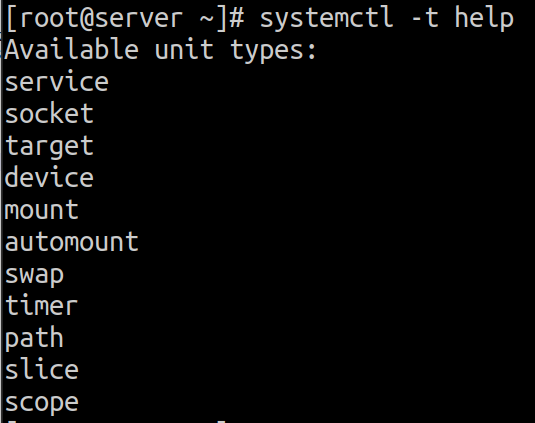
\includegraphics[scale=.5]{content/chapter1/images/units.png}
			\caption{Sample output}
			\label{fig:mascot}
		\end{figure}	
	
		\item Command to list all units of a specific type:		
		\begin{tcolorbox}[breakable,notitle,boxrule=1pt,colback=black,colframe=black]
			\color{green}
			\fontdimen2\font=1em
			\# systemctl ---type=service
			\newline
			\# systemctl ---type=socket
			\newline
			\# systemctl ---type=mount
			\fontdimen2\font=4pt
		\end{tcolorbox}
		
	\end{itemize}
		

	\newpage
	

	\textbf{Location of systemd units file:}
	\begin{itemize}
		\item \textbf{/usr/lib/systemd/system/}
		\item \textbf{/etc/systemd/system/}
	\end{itemize}
	
	\textbf{Some common unit types are listed as follows:}
	\begin{itemize}
		\item \textbf{Service units}:
		\begin{itemize}
			\item Service units represent system services.
			\item They have a \textbf{".service"} extension.
			\item Used to start/stop/restart/reload daemons, such as a web server.
			\item Eg: sshd.service unit file is at /usr/lib/systemd/system/sshd.service
		\end{itemize}
		\bigskip\bigskip
		\item \textbf{Socket units}:
		\begin{itemize}
			\item What is a socket? A socket consists of the IP address of a system and the port number of a program within the system. 
			\begin{figure}[h!]
				\centering
				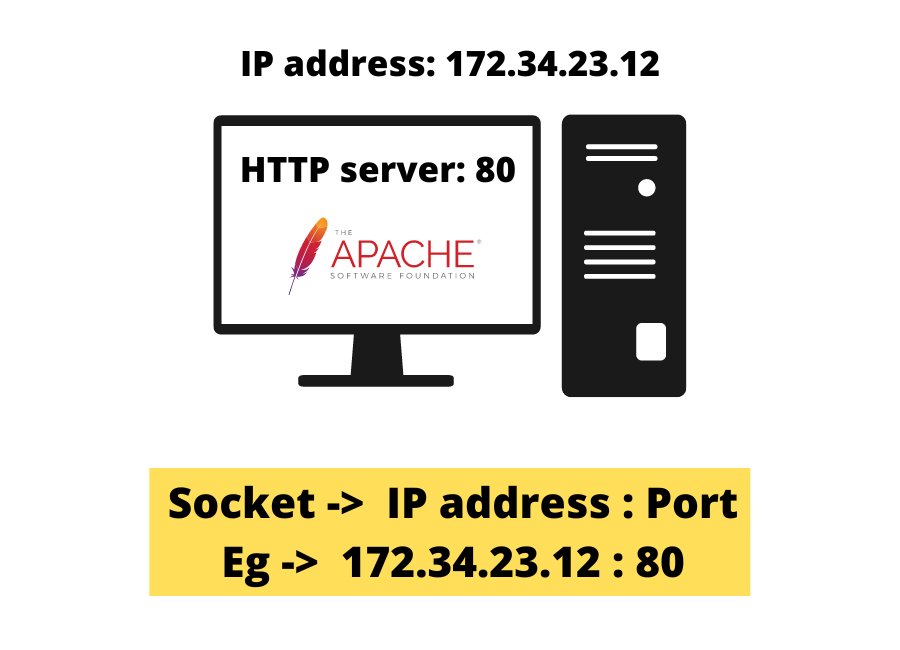
\includegraphics[scale=0.4]{content/chapter1/images/socket.png}
				\caption{Socket}
				\label{fig:socket1}
			\end{figure}
			\item A socket unit listen on an IP address and a port, and when something connects to it, the socket is handed over to the daemon it is made for.
			\item They have a \textbf{".socket"} extension.
			\item They represent interprocess communication (IPC) sockets.	
			\item Eg: dbus.socket unit file is at /usr/lib/systemd/system/dbus.socket
		\end{itemize}
		\bigskip \bigskip
		\item \textbf{Target units}:
		\begin{itemize}
			\item Targets are used for grouping and ordering units. 
			\item At different targets, different services, sockets, and other units are started.
			\item They have a \textbf{".target"} extension.
			\item Eg: multi-user.target unit file is at /usr/lib/systemd/system/multi-user.target
		\end{itemize}
		

	\end{itemize}
	
\end{flushleft}

\newpage


\subsection{systemctl to manage services}
\setlength{\columnsep}{20pt}
\begin{flushleft}



	\begin{tabulary}{1.0\textwidth}{|p{13em}|p{13em}|}
			\toprule
			\textbf{Command} & \textbf{Purpose}\\
			\midrule
			\textbf{systemctl start service} \newline \bigskip Eg: \color{blue} \textbf{systemctl start sshd}  & Start a service/daemon. \\
			\hline
			\textbf{systemctl status service} \newline \bigskip Eg: \color{blue} \textbf{systemctl status sshd}  & Display status of a service/daemon. \\
			\hline
			\textbf{systemctl stop service} \newline \bigskip Eg: \color{blue} \textbf{systemctl stop sshd}  & Stop a service/daemon. \\
			\hline
			\textbf{systemctl restart service} \newline \bigskip Eg: \color{blue} \textbf{systemctl restart sshd}  & Restart a service/daemon.  The PID of daemon will change.	\\
			\hline
			\textbf{systemctl reload service} \newline \bigskip Eg: \color{blue} \textbf{systemctl restart sshd}  & Restart a service/daemon.  The PID of daemon will change.	\\
			\hline
			\textbf{systemctl reload service} \newline \bigskip Eg: \color{blue} \textbf{systemctl restart sshd}  & Reload a service/daemon. The process ID of daemon will not change.	 \\
			\hline
			\textbf{systemctl enable service} \newline \bigskip Eg: \color{blue} \textbf{systemctl enable sshd}  & Enables a service/daemon permanently, which means service/daemon will automatically start on system boot up. \\
			\hline
			\textbf{systemctl disable service} \newline \bigskip Eg: \color{blue} \textbf{systemctl enable sshd}  & Disable a service/daemon permanently, which means service/daemon will not automatically start on system boot up. \\
			\hline
			\textbf{systemctl list-dependencies service} \newline \bigskip Eg: \color{blue} \textbf{systemctl list-dependencies sshd}  & List units which are required and wanted by
			the specified unit. \\
			\bottomrule
	\end{tabulary}




\end{flushleft}

\newpage


\subsection{systemctl to manage targets}
\setlength{\columnsep}{20pt}
\begin{flushleft}

	\begin{tabulary}{1.0\textwidth}{|p{10em}|p{16em}|}
			\toprule
			\textbf{Systemd targets} & \textbf{Purpose}\\
			\midrule
			\textbf{graphical.target} & System supports multiple users, graphical and text-based logins. \\
			\hline
			\textbf{multi-user.target} & System supports multiple users, text-based logins only. \\
			\hline
			\textbf{rescue.target} & sulogin prompt, basic system initialization completed. \\
			\hline
			\textbf{emergency.target} & sulogin prompt, initramfs pivot complete and system root mounted on / read-only.	\\
			\bottomrule
	\end{tabulary}

	Commands to manage targets:

	\begin{tabulary}{1.0\textwidth}{|p{13em}|p{13em}|}
		\toprule
		\textbf{Command} & \textbf{Purpose}\\
		\midrule
		\textbf{systemctl set-default target} \newline Eg: \color{blue} \textbf{systemctl set-default graphical.target} \bigskip   & Set a default target/runlevel so that the system boots into that specific target. \\
		\hline
		\textbf{systemctl get-default} \bigskip & Get default target/runlevel. \\
		\hline
		\textbf{systemctl isolate target} \newline Eg: \color{blue} \textbf{systemctl isolate multi-user.target} \bigskip   & Switch to a specific target instantly. \\
		\bottomrule
	\end{tabulary}


	


\end{flushleft}

\newpage


\subsection{Selecting target at boot time}
\begin{flushleft}

	\bigskip
		\begin{enumerate}
			\item (Re)boot the system.
			\item Interrupt the boot loader menu countdown by pressing any key.
			\item Move the cursor to the entry to be started.
			\item \textbf{Press e} to edit the current entry.
			\item Move the cursor to the line that starts with \textbf{linux}. This is the kernel command line.
			\item Append \textbf{systemd.unit=desired.target}.
			\newline eg: systemd.unit=multi-user.target
			
			\begin{figure}[h!]
				\centering
				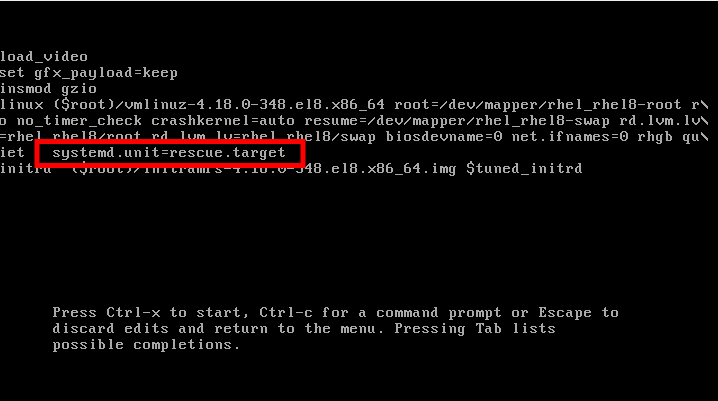
\includegraphics[scale=.5]{content/chapter1/images/rescue.png}
				\caption{Sample output}
				\label{fig:free_h_s_2}
			\end{figure}
			
			\item Press \textbf{Ctrl+x} to boot with these changes.
		\end{enumerate}
	
\end{flushleft}

\newpage
\subsection{Recovering the root password}
\begin{flushleft}
	\begin{itemize}

		\begin{enumerate}
			\item (Re)boot the system.
			\item Interrupt the boot loader menu countdown by pressing any key.
			\item Move the cursor to the entry to be started.
			\item \textbf{Press e} to edit the current entry.
			\item Move the cursor to the line that starts with linux16. This is the kernel command line.
			\item Append \textbf{rd.break} (this will break just before control is handed from the initramfs to the actual system).
			\item Press \textbf{Ctrl+x} to boot with these changes.
		\end{enumerate}
		At this point, a root shell will be presented, with the root file system for the actual system 	mounted read-only on /sysroot.
		\newline
		\newline
		To recover the root password from this point, use the following procedure:
		
		\begin{enumerate}
			\item Remount /sysroot as read-write.
			\begin{tcolorbox}[breakable,notitle,boxrule=-0pt,colback=black,colframe=black]
				\color{green}
				\fontdimen2\font=1em
				switch\_root:/\# \textbf{mount -o remount,rw /sysroot}
				\fontdimen2\font=4pt
			\end{tcolorbox}
			\item Switch into a chroot jail, where /sysroot is treated as the root of the file system tree.
			\begin{tcolorbox}[breakable,notitle,boxrule=-0pt,colback=black,colframe=black]
				\color{green}
				\fontdimen2\font=1em
				switch\_root:/\# \textbf{chroot /sysroot}
				\fontdimen2\font=4pt
			\end{tcolorbox}
			\item Set a new root password:
			\begin{tcolorbox}[breakable,notitle,boxrule=-0pt,colback=black,colframe=black]
				\color{green}
				\fontdimen2\font=1em
				sh-4.2\# \textbf{passwd root}
				\fontdimen2\font=4pt
			\end{tcolorbox}
			\item Make sure that all unlabeled files (including /etc/shadow at this point) get relabeled during boot.
			\begin{tcolorbox}[breakable,notitle,boxrule=-0pt,colback=black,colframe=black]
				\color{green}
				\fontdimen2\font=1em
				sh-4.2\# \textbf{touch /.autorelabel}
				\fontdimen2\font=4pt
			\end{tcolorbox}
		
			\item Type \textbf{exit} twice. The first will exit the \textbf{chroot} jail, and the second will exit the initramfs debug shell.
		\end{enumerate}
	
		At this point, the system will continue booting, perform a full SELinux relabel, then reboot again.
	\end{itemize}
\end{flushleft}

\newpage
\subsection{Troubleshooting boot issues}
\begin{flushleft}
	If your system is getting stuck during system boot, you can troubleshoot the system by booting it into rescue or emergency mode:
\bigskip
\begin{itemize}
	\item Append either \textbf{systemd.unit=rescue.target} or \textbf{systemd.unit=emergency.target} to the kernel command line to boot the system into a  rescue or emergency shell instead of starting normally. 
	\item Both of these shells require the root password. 
	\item The \textbf{emergency.target} keeps the root file system mounted read-only.
	\begin{figure}[h!]
		\centering
		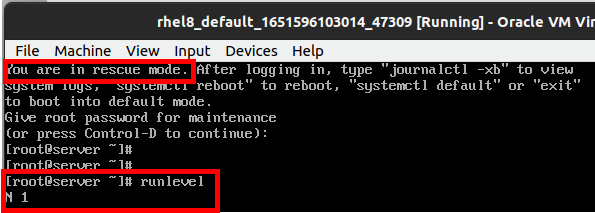
\includegraphics[scale=.6]{content/chapter1/images/emer.png}
		\caption{Sample output}
		\label{fig:free_h_s_2_3}
	\end{figure}
	
	\item The \textbf{rescue.target} waits for sysinit.target to complete first so that more of the system will be initialized, for example, logging, file systems, etc. 
	\begin{figure}[h!]
		\centering
		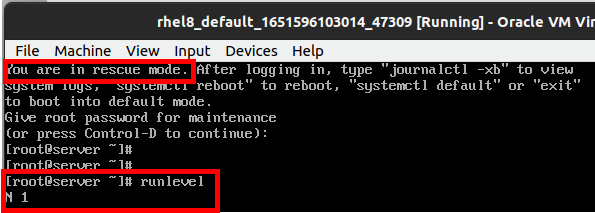
\includegraphics[scale=.6]{content/chapter1/images/rescue2.png}
		\caption{Sample output}
		\label{fig:free_h_s_2_4}
	\end{figure}
	
	\item Exiting from these shells will continue with the regular boot process.
\end{itemize}
\end{flushleft}

\newpage
\subsection{Practice}\index{Linux directory structure!Practice}
\setlength{\columnsep}{3pt}
\begin{flushleft}

	\begin{itemize}
		\item List all the available zones:
		\begin{tcolorbox}[breakable,notitle,boxrule=1pt,colback=pink,colframe=pink]
			\color{black}
			\fontdimen2\font=1em
			Syntax: firewall-cmd --get-zones
			\fontdimen2\font=4pt
		\end{tcolorbox}	
		Eg:
		\begin{figure}[h!]
			\centering
			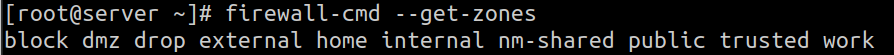
\includegraphics[scale=0.4]{content/chapter2/images/zones.png}
			\caption{Sample output}
			\label{fig:zones}
		\end{figure}
		
		\bigskip
		\bigskip
		
		\item Display the default zones:
		\begin{tcolorbox}[breakable,notitle,boxrule=1pt,colback=pink,colframe=pink]
			\color{black}
			\fontdimen2\font=1em
			Syntax: firewall-cmd --get-default-zone
			\fontdimen2\font=4pt
		\end{tcolorbox}	
		Eg:
		\begin{figure}[h!]
			\centering
			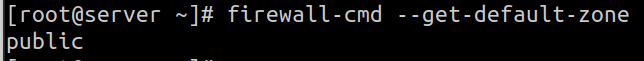
\includegraphics[scale=0.5]{content/chapter2/images/zones2.png}
			\caption{Sample output}
			\label{fig:zones2}
		\end{figure}

		\bigskip
		\bigskip

		\item Set the default zone:
		\begin{tcolorbox}[breakable,notitle,boxrule=1pt,colback=pink,colframe=pink]
			\color{black}
			\fontdimen2\font=1em
			Syntax: firewall-cmd --set-default-zone=<zone>
			\fontdimen2\font=4pt
		\end{tcolorbox}	
		Eg:
		\begin{figure}[h!]
			\centering
			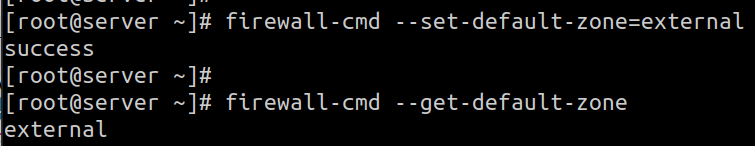
\includegraphics[scale=0.45]{content/chapter2/images/zones3.png}
			\caption{Sample output}
			\label{fig:zones3}
		\end{figure}

		\newpage

		\item Display information for all zones (interfaces, sources, ports, services, etc).
		\bigskip
		\begin{tcolorbox}[breakable,notitle,boxrule=1pt,colback=pink,colframe=pink]
			\color{black}
			\fontdimen2\font=1em
			Syntax: firewall-cmd ---list-all-zones
			\fontdimen2\font=4pt
		\end{tcolorbox}	

		\bigskip
		\bigskip		
		
		\item Display information for specific zone (interfaces, sources, ports, services, etc). If no \textbf{"--zone="} option is provided, the default zone will be used.
		\bigskip
		\begin{tcolorbox}[breakable,notitle,boxrule=1pt,colback=pink,colframe=pink]
			\color{black}
			\fontdimen2\font=1em
			Syntax: firewall-cmd ---list-all [--zone=<ZONE>]
			\fontdimen2\font=4pt
		\end{tcolorbox}	
		Eg:
		\begin{figure}[h!]
			\centering
			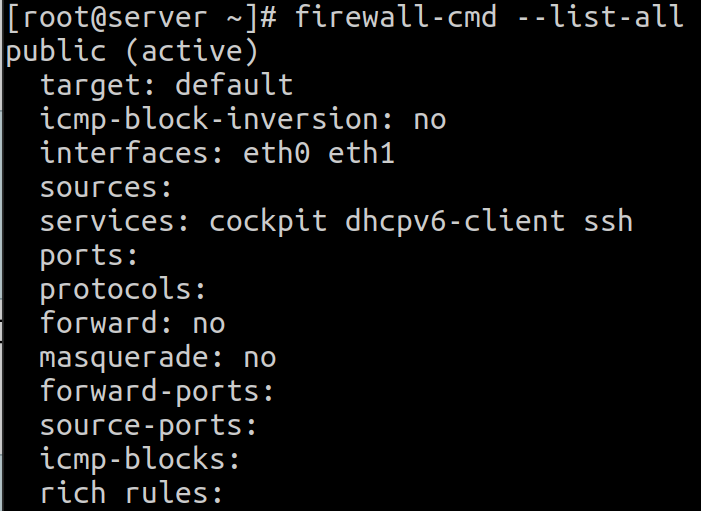
\includegraphics[scale=0.4]{content/chapter2/images/zones5.png}
			\caption{Sample output}
			\label{fig:zones4}
		\end{figure}

		\newpage
		\item Apply changes done by \textbf{firewall-cmd} command immediately:
		\begin{tcolorbox}[breakable,notitle,boxrule=1pt,colback=pink,colframe=pink]
			\color{black}
			\fontdimen2\font=1em
			Syntax: firewall-cmd ---reload
			\fontdimen2\font=4pt
		\end{tcolorbox}	
		
		\bigskip
		\bigskip
		
		\item Allow traffic to <SERVICE>. If no --zone= option is provided, the default zone will be used.
		\bigskip
		\begin{tcolorbox}[breakable,notitle,boxrule=1pt,colback=pink,colframe=pink]
			\color{black}
			\fontdimen2\font=1em
			Syntax: 
			\newline
			firewall-cmd ---add-service=<service> ---permanent [--zone=<ZONE>]
			\newline
			\newline
			firewall-cmd ---reload
			\fontdimen2\font=4pt
		\end{tcolorbox}	
		Eg:
		\begin{tcolorbox}[breakable,notitle,boxrule=-0pt,colback=black,colframe=black]
			\color{green}
			\fontdimen2\font=1em
			\# firewall-cmd --add-service=httpd --permanent 
			\newline
			\# firewall-cmd --reload
			\fontdimen2\font=4pt
		\end{tcolorbox}
		\begin{figure}[h!]
			\centering
			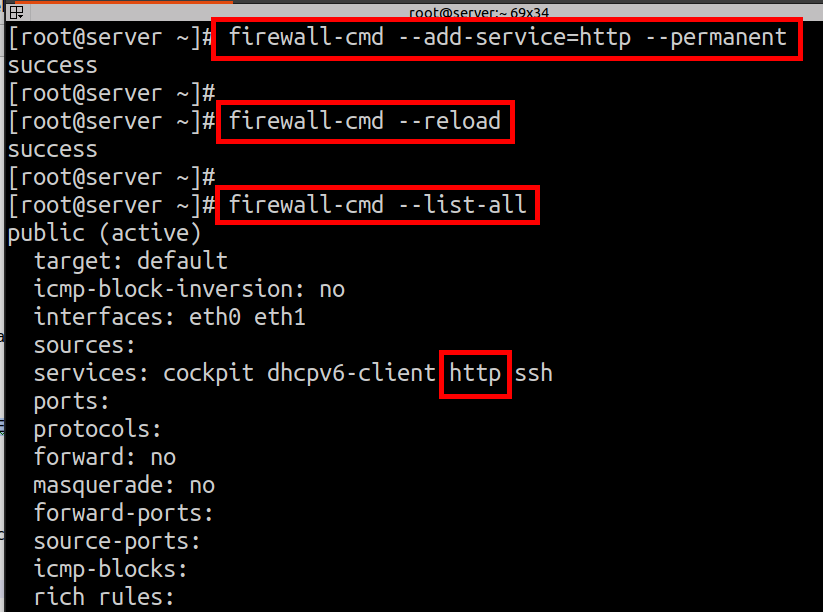
\includegraphics[scale=0.4]{content/chapter2/images/zones6.png}
			\caption{Sample output}
			\label{fig:zones6}
		\end{figure}
		\newpage
		
		\item Remove <SERVICE> from the allowed list for the zone. If no \textbf{"--zone="} option is provided, the default zone will be used.
		\bigskip
		\begin{tcolorbox}[breakable,notitle,boxrule=1pt,colback=pink,colframe=pink]
			\color{black}
			\fontdimen2\font=1em
			Syntax: 
			\newline
			firewall-cmd ---remove-service=<service> ---permanent [--zone=<ZONE>]
			\newline
			\newline
			firewall-cmd ---reload
			\fontdimen2\font=4pt
		\end{tcolorbox}	
		Eg:
		\begin{tcolorbox}[breakable,notitle,boxrule=-0pt,colback=black,colframe=black]
			\color{green}
			\fontdimen2\font=1em
			\# firewall-cmd --remove-service=httpd --permanent 
			\newline
			\# firewall-cmd --reload
			\fontdimen2\font=4pt
		\end{tcolorbox}
		\begin{figure}[h!]
			\centering
			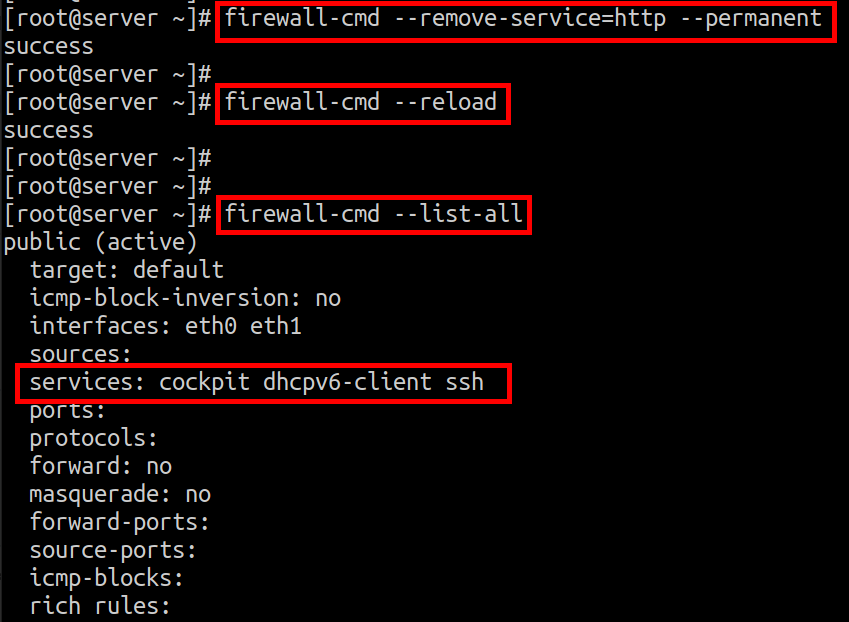
\includegraphics[scale=0.4]{content/chapter2/images/zones7.png}
			\caption{Sample output}
			\label{fig:zones7}
		\end{figure}
		
		\newpage
		\item Allow traffic to the \textbf{<PORT/PROTOCOL>} port(s). If no \textbf{"--zone="} option is provided, the default zone will be used.
		\bigskip
		\begin{tcolorbox}[breakable,notitle,boxrule=1pt,colback=pink,colframe=pink]
			\color{black}
			\fontdimen2\font=1em
			Syntax: 
			\newline
			firewall-cmd ---add-port=<PORT/PROTOCOL> ---permanent [--zone=<ZONE>]
			\newline
			\newline
			firewall-cmd ---reload
			\fontdimen2\font=4pt
		\end{tcolorbox}	
		Eg:
		\begin{tcolorbox}[breakable,notitle,boxrule=-0pt,colback=black,colframe=black]
			\color{green}
			\fontdimen2\font=1em
			\# firewall-cmd --add-port=6060/tcp --permanent 
			\newline
			\# firewall-cmd --reload
			\fontdimen2\font=4pt
		\end{tcolorbox}
		\begin{figure}[h!]
			\centering
			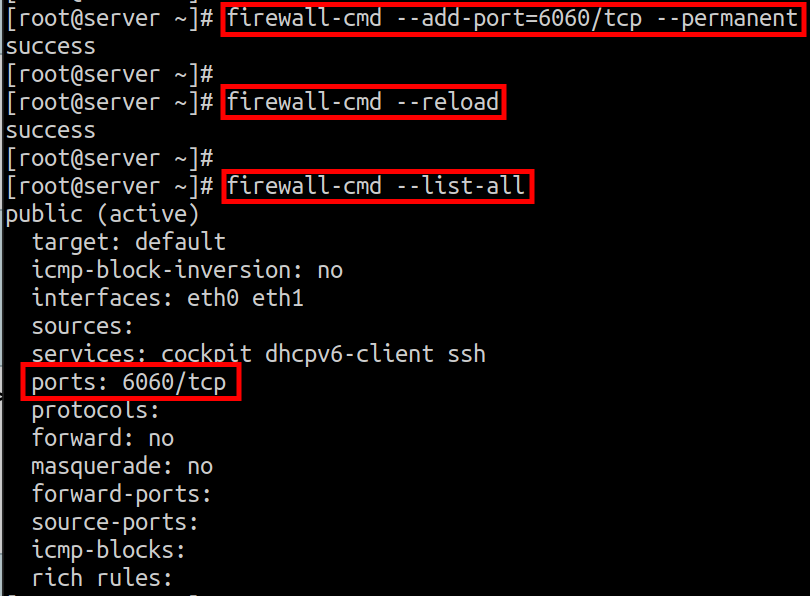
\includegraphics[scale=0.4]{content/chapter2/images/zones8.png}
			\caption{Sample output}
			\label{fig:zones8}
		\end{figure}
		
		\newpage
		\item Remove the <PORT/PROTOCOL> port(s) from the allowed list for the zone. If no \textbf{"--zone="} option is provided, the default zone will be used.
		\bigskip
		\begin{tcolorbox}[breakable,notitle,boxrule=1pt,colback=pink,colframe=pink]
			\color{black}
			\fontdimen2\font=1em
			Syntax: 
			\newline
			firewall-cmd ---remove-port=<PORT/PROTOCOL> ---permanent [--zone=<ZONE>]
			\newline
			\newline
			firewall-cmd ---reload
			\fontdimen2\font=4pt
		\end{tcolorbox}	
		Eg:
		\begin{tcolorbox}[breakable,notitle,boxrule=-0pt,colback=black,colframe=black]
			\color{green}
			\fontdimen2\font=1em
			\# firewall-cmd --remove-port=6060/tcp --permanent 
			\newline
			\# firewall-cmd --reload
			\fontdimen2\font=4pt
		\end{tcolorbox}
		\begin{figure}[h!]
			\centering
			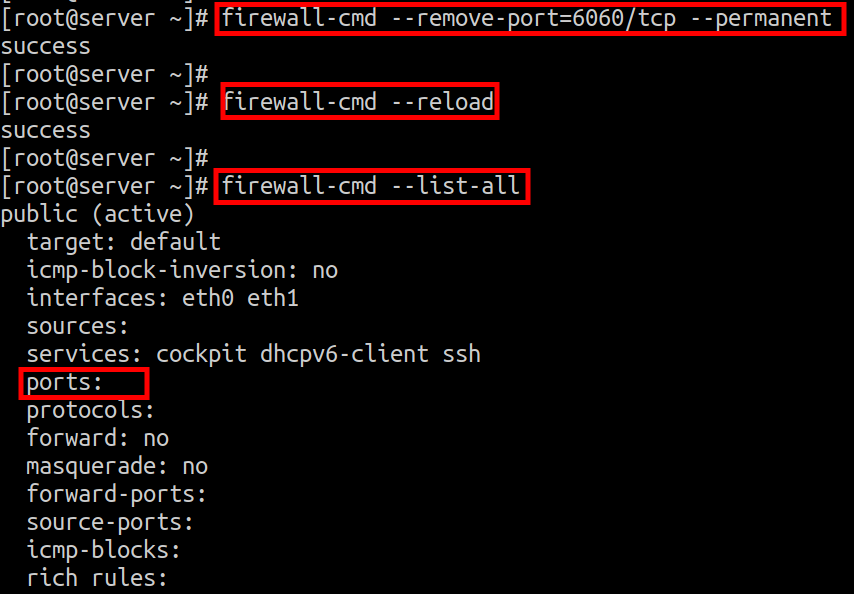
\includegraphics[scale=0.4]{content/chapter2/images/zones9.png}
			\caption{Sample output}
			\label{fig:zones9}
		\end{figure}
			
		
		
	\end{itemize}
	
\end{flushleft}
\newpage

%-----------------------

%--------------------------------------------------------------------------
%	CHAPTER 2
%-------------------------------------------------------------------------

\chapterimage{index3.png} % Table of contents heading image
\chapter{Firewall in Linux}
%-----------------------
\section{firewalld in detail}
\setlength{\columnsep}{3pt}
\begin{flushleft}
	\bigskip
	\bigskip
	\begin{tcolorbox}[breakable,notitle,boxrule=1pt,colback=black,colframe=black]
		\color{white}
		\bigskip
		In this section, you are going to learn:
		\begin{enumerate}
			\item \textbf{Filesystem Hierarchy Standard (FHS)}
			\item \textbf{Important directories in FHS}
			\item \textbf{Some shortcuts to use in Linux OS}
		\end{enumerate}	
		\bigskip
		Finally, there will be a \textbf{small excerise} on these topics to check your knowledge.
		\bigskip
	\end{tcolorbox}
	
	
	\bigskip
	\bigskip
	
	\begin{multicols}{2}
		\vspace*{\fill}
		\vspace*{\fill}
		\vspace*{\fill}
		\vspace*{\fill}
		\vspace*{\fill}
		\vspace*{\fill}
		\vspace*{\fill}
		\vspace*{\fill}
		\vspace*{\fill}
		
		\vfill \null
		\columnbreak
		So let's get started....
		
\includegraphics[scale=0.08]{content/linux_section.png}
	\end{multicols}	
	
\end{flushleft}

\newpage






\subsection{Firewall overview}

\begin{flushleft}
	\begin{itemize}
		\item A firewall is a security system that prevent unauthorized access to a computer network. 
		\item \textbf{Firewalls guard traffic at a computer's ports}, where information is exchanged with external devices.
	
	
	\bigskip
	\bigskip
	\begin{figure}[h!]
		\centering
		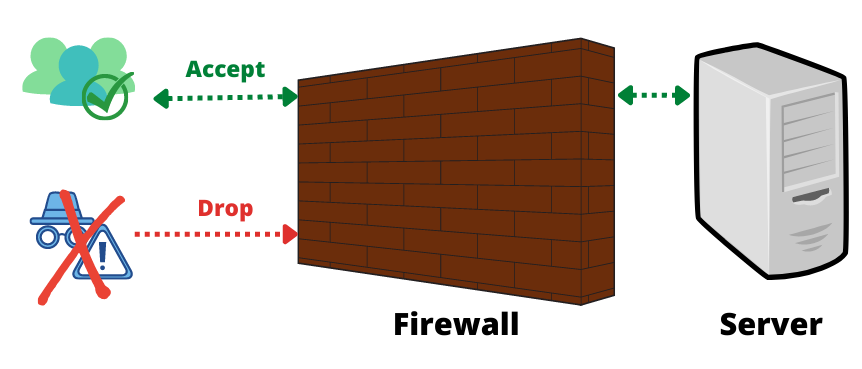
\includegraphics[scale=.5]{content/chapter2/images/firewall.png}
		\caption{Firewall}
		\label{fig:firewall}
	\end{figure}

	\bigskip
	
	\item \textbf{firewalld} is the deamon for firewall in RHEL.
	\item Service unit for this daemon is \textbf{firewalld.service}.
	
	\end{itemize}
	
\end{flushleft}

\newpage


\subsection{firewalld zones}

\begin{flushleft}
	
	\begin{itemize}
		\item The firewalld separates all incoming traffic into zones.
		\item Each zone have its own set of rules.
		\item Below are predefined zones with firewalld, having different usage:
		\bigskip
			\begin{tabulary}{1.0\textwidth}{|p{13em}|p{13em}|}
			\toprule
			\textbf{Zone name} & \textbf{Default configuration}\\
			\midrule
			\textbf{trusted} & Allow all incoming traffic. \\
			\hline
			\textbf{home} & Reject incoming traffic except the ssh, mdns, ipp-client, samba-client, or dhcpv6-client services \\
			\hline
			\textbf{internal} & Reject incoming traffic except ssh, ipp-client, or dhcpv6-client services. \\
			\hline
			\textbf{public} & Reject incoming traffic ssh or dhcpv6-client services. \\
			\hline
			\textbf{external} & Reject incoming traffic except ssh service. Masqueraded IPv4
			address of the outgoing network interface. \\
			\hline
			\textbf{dmz} & Reject incoming traffic except outgoing traffic for ssh service. \\
			\hline
			\textbf{block}  & Reject all incoming traffic unless related to outgoing traffic. \\
			\hline
			\textbf{drop} & Drop all incoming traffic unless related to outgoing traffic (do not even respond with ICMP errors). \\
			\bottomrule
		\end{tabulary}
		\item The \textbf{public zone} is the default zone for network interfaces.
	\end{itemize}
	
\end{flushleft}

\newpage

\subsection{firewall-cmd command}
\setlength{\columnsep}{3pt}
\begin{flushleft}

	\begin{itemize}
		\item List all the available zones:
		\begin{tcolorbox}[breakable,notitle,boxrule=1pt,colback=pink,colframe=pink]
			\color{black}
			\fontdimen2\font=1em
			Syntax: firewall-cmd --get-zones
			\fontdimen2\font=4pt
		\end{tcolorbox}	
		Eg:
		\begin{figure}[h!]
			\centering
			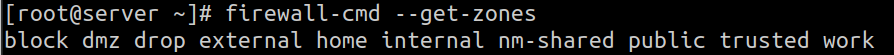
\includegraphics[scale=0.4]{content/chapter2/images/zones.png}
			\caption{Sample output}
			\label{fig:zones}
		\end{figure}
		
		\bigskip
		\bigskip
		
		\item Display the default zones:
		\begin{tcolorbox}[breakable,notitle,boxrule=1pt,colback=pink,colframe=pink]
			\color{black}
			\fontdimen2\font=1em
			Syntax: firewall-cmd --get-default-zone
			\fontdimen2\font=4pt
		\end{tcolorbox}	
		Eg:
		\begin{figure}[h!]
			\centering
			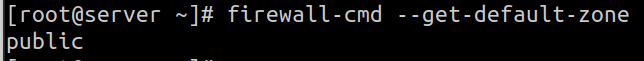
\includegraphics[scale=0.5]{content/chapter2/images/zones2.png}
			\caption{Sample output}
			\label{fig:zones2}
		\end{figure}

		\bigskip
		\bigskip

		\item Set the default zone:
		\begin{tcolorbox}[breakable,notitle,boxrule=1pt,colback=pink,colframe=pink]
			\color{black}
			\fontdimen2\font=1em
			Syntax: firewall-cmd --set-default-zone=<zone>
			\fontdimen2\font=4pt
		\end{tcolorbox}	
		Eg:
		\begin{figure}[h!]
			\centering
			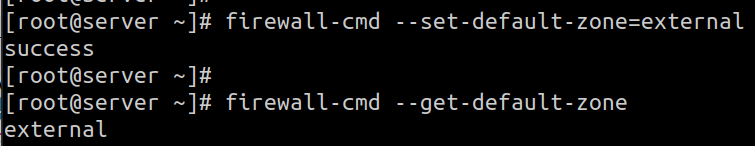
\includegraphics[scale=0.45]{content/chapter2/images/zones3.png}
			\caption{Sample output}
			\label{fig:zones3}
		\end{figure}

		\newpage

		\item Display information for all zones (interfaces, sources, ports, services, etc).
		\bigskip
		\begin{tcolorbox}[breakable,notitle,boxrule=1pt,colback=pink,colframe=pink]
			\color{black}
			\fontdimen2\font=1em
			Syntax: firewall-cmd ---list-all-zones
			\fontdimen2\font=4pt
		\end{tcolorbox}	

		\bigskip
		\bigskip		
		
		\item Display information for specific zone (interfaces, sources, ports, services, etc). If no \textbf{"--zone="} option is provided, the default zone will be used.
		\bigskip
		\begin{tcolorbox}[breakable,notitle,boxrule=1pt,colback=pink,colframe=pink]
			\color{black}
			\fontdimen2\font=1em
			Syntax: firewall-cmd ---list-all [--zone=<ZONE>]
			\fontdimen2\font=4pt
		\end{tcolorbox}	
		Eg:
		\begin{figure}[h!]
			\centering
			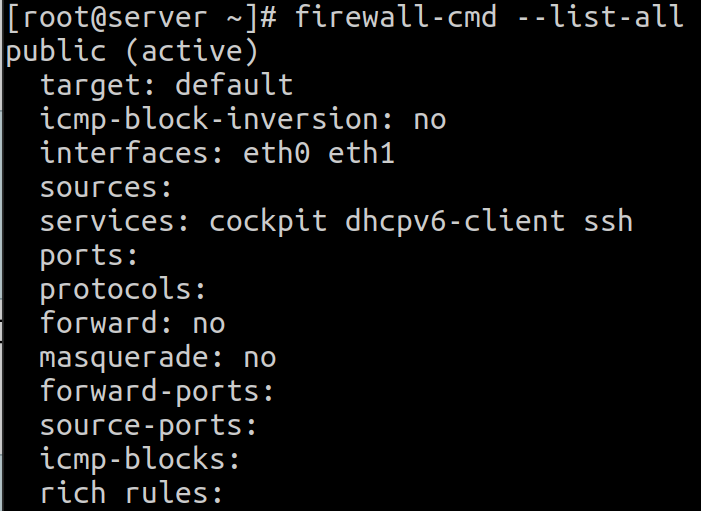
\includegraphics[scale=0.4]{content/chapter2/images/zones5.png}
			\caption{Sample output}
			\label{fig:zones4}
		\end{figure}

		\newpage
		\item Apply changes done by \textbf{firewall-cmd} command immediately:
		\begin{tcolorbox}[breakable,notitle,boxrule=1pt,colback=pink,colframe=pink]
			\color{black}
			\fontdimen2\font=1em
			Syntax: firewall-cmd ---reload
			\fontdimen2\font=4pt
		\end{tcolorbox}	
		
		\bigskip
		\bigskip
		
		\item Allow traffic to <SERVICE>. If no --zone= option is provided, the default zone will be used.
		\bigskip
		\begin{tcolorbox}[breakable,notitle,boxrule=1pt,colback=pink,colframe=pink]
			\color{black}
			\fontdimen2\font=1em
			Syntax: 
			\newline
			firewall-cmd ---add-service=<service> ---permanent [--zone=<ZONE>]
			\newline
			\newline
			firewall-cmd ---reload
			\fontdimen2\font=4pt
		\end{tcolorbox}	
		Eg:
		\begin{tcolorbox}[breakable,notitle,boxrule=-0pt,colback=black,colframe=black]
			\color{green}
			\fontdimen2\font=1em
			\# firewall-cmd --add-service=httpd --permanent 
			\newline
			\# firewall-cmd --reload
			\fontdimen2\font=4pt
		\end{tcolorbox}
		\begin{figure}[h!]
			\centering
			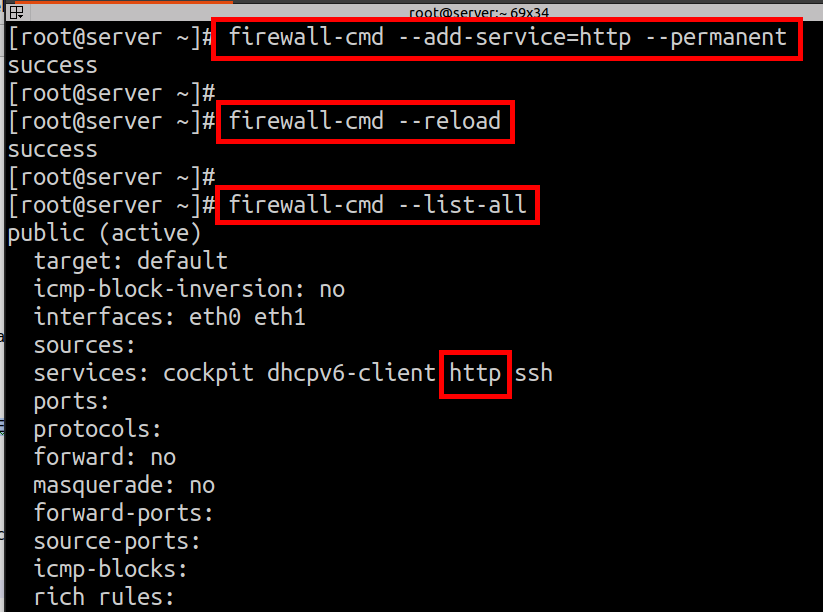
\includegraphics[scale=0.4]{content/chapter2/images/zones6.png}
			\caption{Sample output}
			\label{fig:zones6}
		\end{figure}
		\newpage
		
		\item Remove <SERVICE> from the allowed list for the zone. If no \textbf{"--zone="} option is provided, the default zone will be used.
		\bigskip
		\begin{tcolorbox}[breakable,notitle,boxrule=1pt,colback=pink,colframe=pink]
			\color{black}
			\fontdimen2\font=1em
			Syntax: 
			\newline
			firewall-cmd ---remove-service=<service> ---permanent [--zone=<ZONE>]
			\newline
			\newline
			firewall-cmd ---reload
			\fontdimen2\font=4pt
		\end{tcolorbox}	
		Eg:
		\begin{tcolorbox}[breakable,notitle,boxrule=-0pt,colback=black,colframe=black]
			\color{green}
			\fontdimen2\font=1em
			\# firewall-cmd --remove-service=httpd --permanent 
			\newline
			\# firewall-cmd --reload
			\fontdimen2\font=4pt
		\end{tcolorbox}
		\begin{figure}[h!]
			\centering
			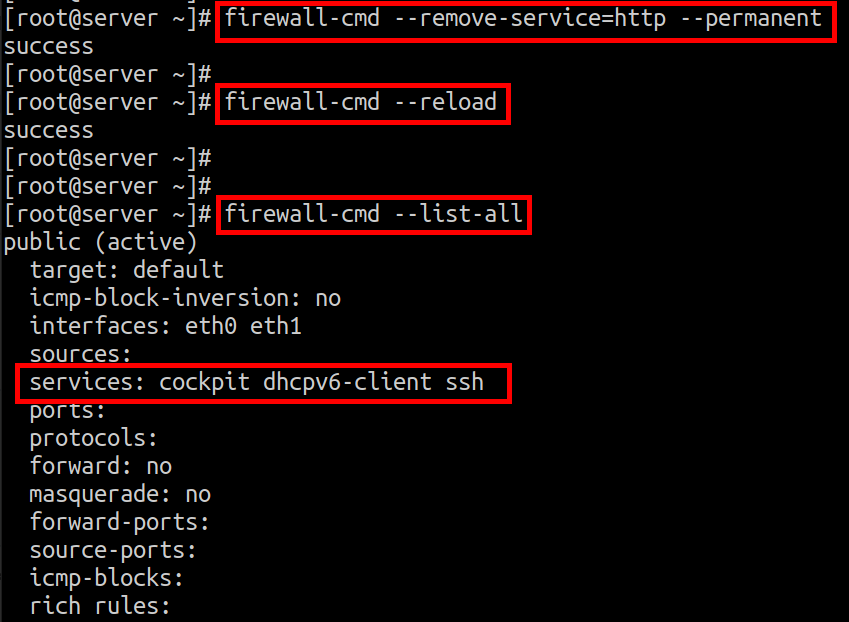
\includegraphics[scale=0.4]{content/chapter2/images/zones7.png}
			\caption{Sample output}
			\label{fig:zones7}
		\end{figure}
		
		\newpage
		\item Allow traffic to the \textbf{<PORT/PROTOCOL>} port(s). If no \textbf{"--zone="} option is provided, the default zone will be used.
		\bigskip
		\begin{tcolorbox}[breakable,notitle,boxrule=1pt,colback=pink,colframe=pink]
			\color{black}
			\fontdimen2\font=1em
			Syntax: 
			\newline
			firewall-cmd ---add-port=<PORT/PROTOCOL> ---permanent [--zone=<ZONE>]
			\newline
			\newline
			firewall-cmd ---reload
			\fontdimen2\font=4pt
		\end{tcolorbox}	
		Eg:
		\begin{tcolorbox}[breakable,notitle,boxrule=-0pt,colback=black,colframe=black]
			\color{green}
			\fontdimen2\font=1em
			\# firewall-cmd --add-port=6060/tcp --permanent 
			\newline
			\# firewall-cmd --reload
			\fontdimen2\font=4pt
		\end{tcolorbox}
		\begin{figure}[h!]
			\centering
			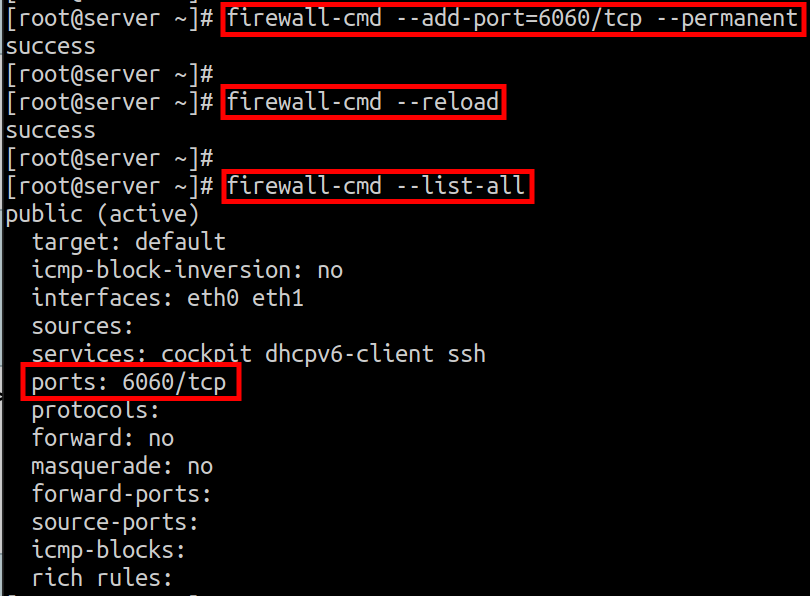
\includegraphics[scale=0.4]{content/chapter2/images/zones8.png}
			\caption{Sample output}
			\label{fig:zones8}
		\end{figure}
		
		\newpage
		\item Remove the <PORT/PROTOCOL> port(s) from the allowed list for the zone. If no \textbf{"--zone="} option is provided, the default zone will be used.
		\bigskip
		\begin{tcolorbox}[breakable,notitle,boxrule=1pt,colback=pink,colframe=pink]
			\color{black}
			\fontdimen2\font=1em
			Syntax: 
			\newline
			firewall-cmd ---remove-port=<PORT/PROTOCOL> ---permanent [--zone=<ZONE>]
			\newline
			\newline
			firewall-cmd ---reload
			\fontdimen2\font=4pt
		\end{tcolorbox}	
		Eg:
		\begin{tcolorbox}[breakable,notitle,boxrule=-0pt,colback=black,colframe=black]
			\color{green}
			\fontdimen2\font=1em
			\# firewall-cmd --remove-port=6060/tcp --permanent 
			\newline
			\# firewall-cmd --reload
			\fontdimen2\font=4pt
		\end{tcolorbox}
		\begin{figure}[h!]
			\centering
			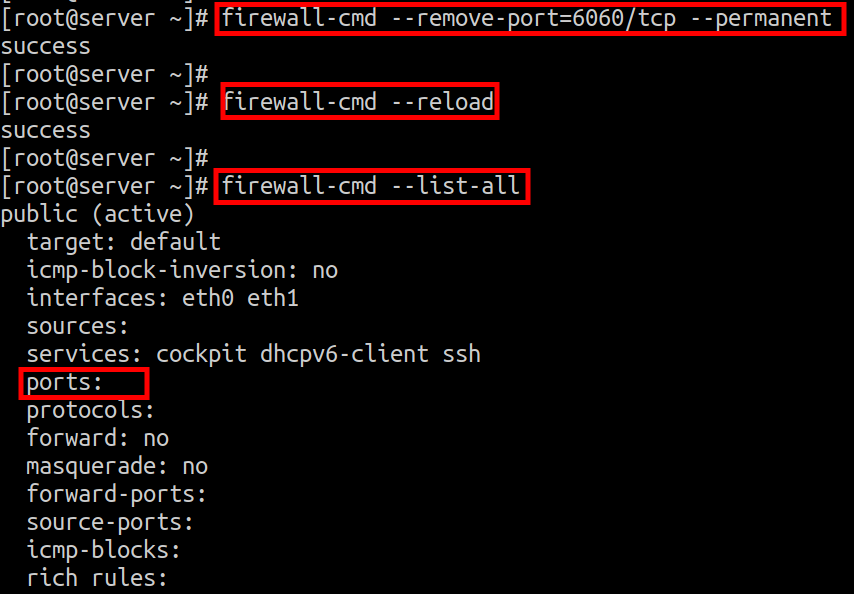
\includegraphics[scale=0.4]{content/chapter2/images/zones9.png}
			\caption{Sample output}
			\label{fig:zones9}
		\end{figure}
			
		
		
	\end{itemize}
	
\end{flushleft}
\newpage

\subsection{Practice}
%\setlength{\columnsep}{3pt}
\begin{flushleft}
	\bigskip
	\bigskip
	\begin{tcolorbox}[breakable,notitle,boxrule=1pt,colback=black,colframe=black]
		\color{white}
		\bigskip
		In this section, you are going to learn:
		\begin{enumerate}
			\item \textbf{Filesystem Hierarchy Standard (FHS)}
			\item \textbf{Important directories in FHS}
			\item \textbf{Some shortcuts to use in Linux OS}
		\end{enumerate}	
		\bigskip
		Finally, there will be a \textbf{small excerise} on these topics to check your knowledge.
		\bigskip
	\end{tcolorbox}
	
	
	\bigskip
	\bigskip
	
	\begin{multicols}{2}
		\vspace*{\fill}
		\vspace*{\fill}
		\vspace*{\fill}
		\vspace*{\fill}
		\vspace*{\fill}
		\vspace*{\fill}
		\vspace*{\fill}
		\vspace*{\fill}
		\vspace*{\fill}
		
		\vfill \null
		\columnbreak
		So let's get started....
		
\includegraphics[scale=0.08]{content/linux_section.png}
	\end{multicols}	
	
\end{flushleft}

\newpage






\section{Advance firewall settings}
\setlength{\columnsep}{3pt}
\begin{flushleft}
	\bigskip
	\bigskip
	\begin{tcolorbox}[breakable,notitle,boxrule=1pt,colback=black,colframe=black]
		\color{white}
		\bigskip
		In this section, you are going to learn:
		\begin{enumerate}
			\item \textbf{Basic commands in Linux OS}
			\item \textbf{Advance commands in Linux OS}
		\end{enumerate}	
		\bigskip
		Finally, there will be a \textbf{small excerise} on these topics to check your knowledge.
		\bigskip
	\end{tcolorbox}
	
	
	\bigskip
	\bigskip
	
	\begin{multicols}{2}
		\vspace*{\fill}
		\vspace*{\fill}
		\vspace*{\fill}
		\vspace*{\fill}
		\vspace*{\fill}
		\vspace*{\fill}
		\vspace*{\fill}
		\vspace*{\fill}
		\vspace*{\fill}
		
		\vfill \null
		\columnbreak
		So let's get started....
		
\includegraphics[scale=0.08]{content/linux_section.png}
	\end{multicols}	
	
\end{flushleft}

\newpage






\subsection{Introduction to rich rules}


\begin{flushleft}
	\begin{itemize}
		\item firewalld rich rules allows custom firewall rules.
		\item Eg: Allow connections to a service from a single IP address, instead of all IP addresses in a zone.
		\item The basic syntax of a rich rule can be expressed by the following block:
		\bigskip
		\begin{tcolorbox}[breakable,notitle,boxrule=0pt,colback=pink,colframe=pink]
			\color{black}
			\fontdimen2\font=1em
			rule
			\newline
   			  [source]
   			\newline
			  [destination]
			\newline
			  service|port|protocol|icmp-block|masquerade|forward-port
			\newline
			  [log]
			\newline
			  [audit]
			\newline
			  [accept|reject|drop]
			\fontdimen2\font=4pt
		\end{tcolorbox}
	\end{itemize}
\end{flushleft}

\newpage


\subsection{Rich rules commands}

\begin{flushleft}
	
	\begin{itemize}
		\item Display all rich rules for the specified zone, or the default zone if no zone is specified.
		\bigskip
		\begin{tcolorbox}[breakable,notitle,boxrule=0pt,colback=pink,colframe=pink]
			\color{black}
			\fontdimen2\font=1em
			Syntax: 
			\newline
			firewall-cmd --list-rich-rules
			\fontdimen2\font=4pt
		\end{tcolorbox}

		\bigskip
		\bigskip
		\item Add <RICH RULE> to the specified zone, or the default zone if no zone is specified.
		\bigskip
		\begin{tcolorbox}[breakable,notitle,boxrule=0pt,colback=pink,colframe=pink]
			\color{black}
			\fontdimen2\font=1em
			Syntax: 
			\newline
			firewall-cmd --permanent --zone=<ZONE> --add-rich-rule='<RULE>'
			\newline
			firewall-cmd --reload
			\fontdimen2\font=4pt
		\end{tcolorbox}
	
		\bigskip
		\bigskip
		\item Remove <RICH RULE> to the specified zone, or the default zone if no zone is specified.
		\bigskip
		\begin{tcolorbox}[breakable,notitle,boxrule=0pt,colback=pink,colframe=pink]
			\color{black}
			\fontdimen2\font=1em
			Syntax: 
			\newline
			firewall-cmd --permanent --zone=<ZONE> --remove-rich-rule='<RULE>'
			\newline
			firewall-cmd --reload
			\fontdimen2\font=4pt
		\end{tcolorbox}
	
	\newpage
	
	\paragraph{Examples:}
	\bigskip
	\begin{enumerate}
		\item Reject all traffic from a "192.168.0.11/32" IP address in default zone:
		\newline
		Eg:
		\begin{tcolorbox}[breakable,notitle,boxrule=-0pt,colback=black,colframe=black]
			\color{green}
			\fontdimen2\font=1em
			\# firewall-cmd --permanent --add-rich-rule='rule family=ipv4 source address=192.168.0.11/32 reject'
			\newline
			\newline
			\# firewall-cmd --reload
			\fontdimen2\font=4pt
		\end{tcolorbox}
		
		\begin{figure}[h!]
			\centering
			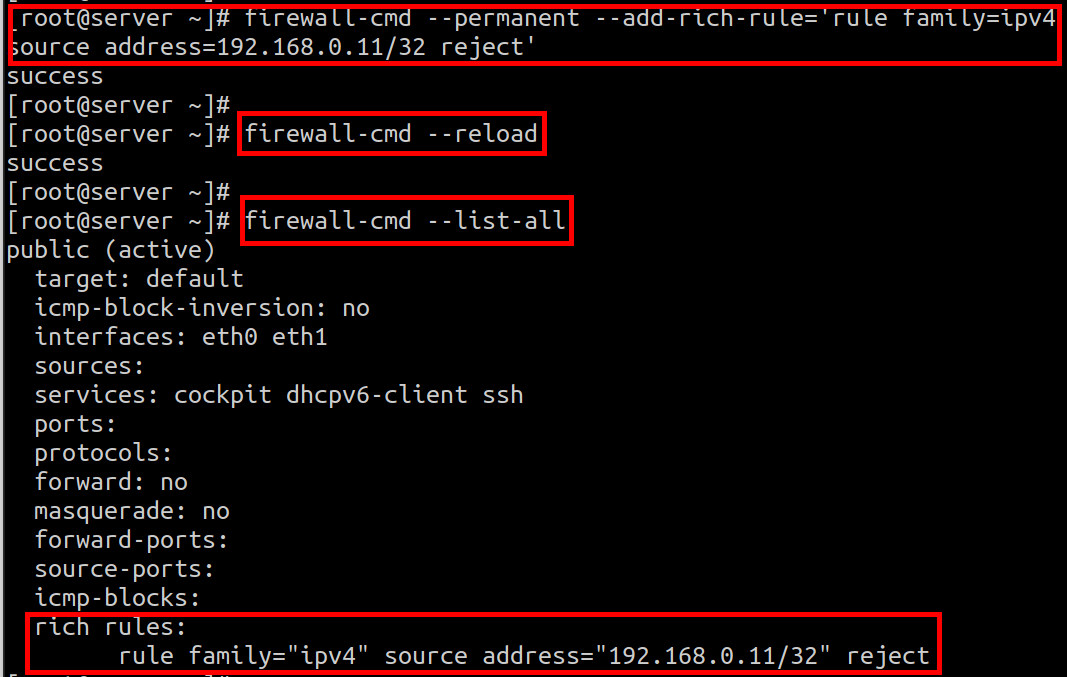
\includegraphics[scale=.3]{content/chapter2/images/zones10.png}
			\caption{Sample output}
			\label{fig:command_prompt7}
		\end{figure}
		
		\newpage
		
		\item Allows port 8080 for a specific IP address "192.168.0.11/32":
		\newline
		Eg:
		\begin{tcolorbox}[breakable,notitle,boxrule=-0pt,colback=black,colframe=black]
			\color{green}
			\fontdimen2\font=1em
			\# firewall-cmd --add-rich-rule='rule family="ipv4" source address="192.168.0.11" port port=8080 protocol=tcp accept'
			\newline
			\newline
			\# firewall-cmd --reload
			\fontdimen2\font=4pt
		\end{tcolorbox}
		
		\begin{figure}[h!]
			\centering
			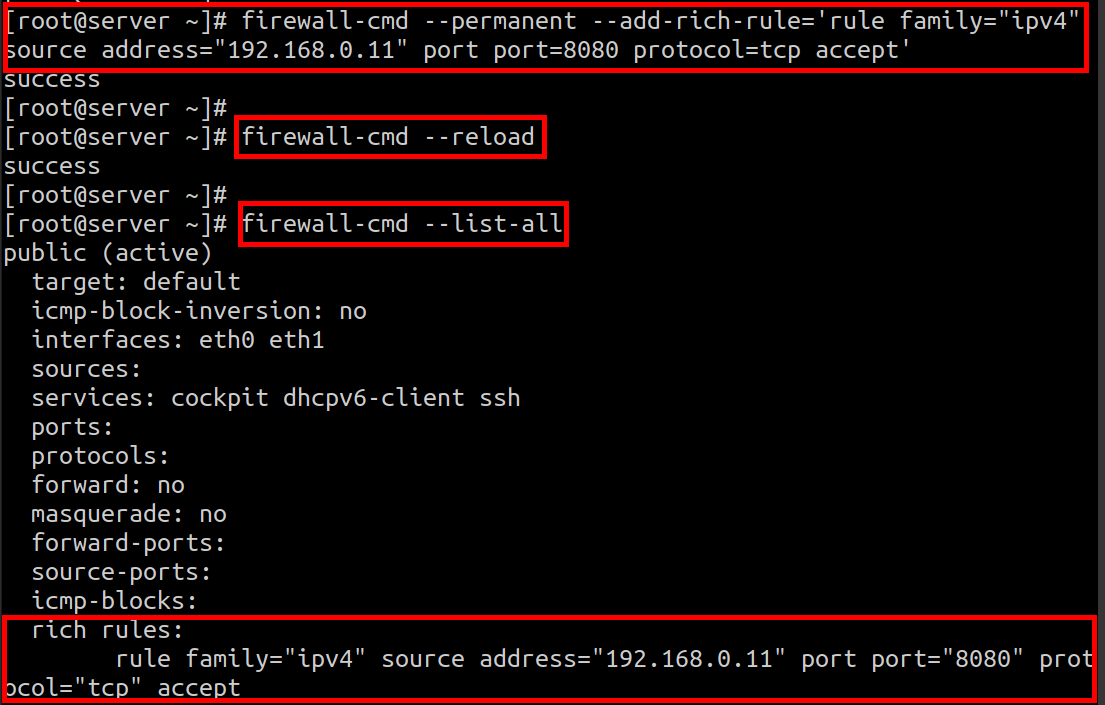
\includegraphics[scale=.3]{content/chapter2/images/zones11.png}
			\caption{Sample output}
			\label{fig:command_prompt9}
		\end{figure}
			
		\newpage
		\item Accept all TCP packets on ports 7900, up to and including port 7905, in the vnc zone for the 192.168.1.0/24 subnet.
		\newline
		Eg:
		\begin{tcolorbox}[breakable,notitle,boxrule=-0pt,colback=black,colframe=black]
			\color{green}
			\fontdimen2\font=1em
			\# firewall-cmd --permanent --zone=vnc --add-rich-rule='rule family=ipv4 source address=192.168.1.0/24 port port=7900-7905 protocol=tcp accept'
			\newline
			\newline
			\# firewall-cmd --reload
			\fontdimen2\font=4pt
		\end{tcolorbox}
		
		\begin{figure}[h!]
			\centering
			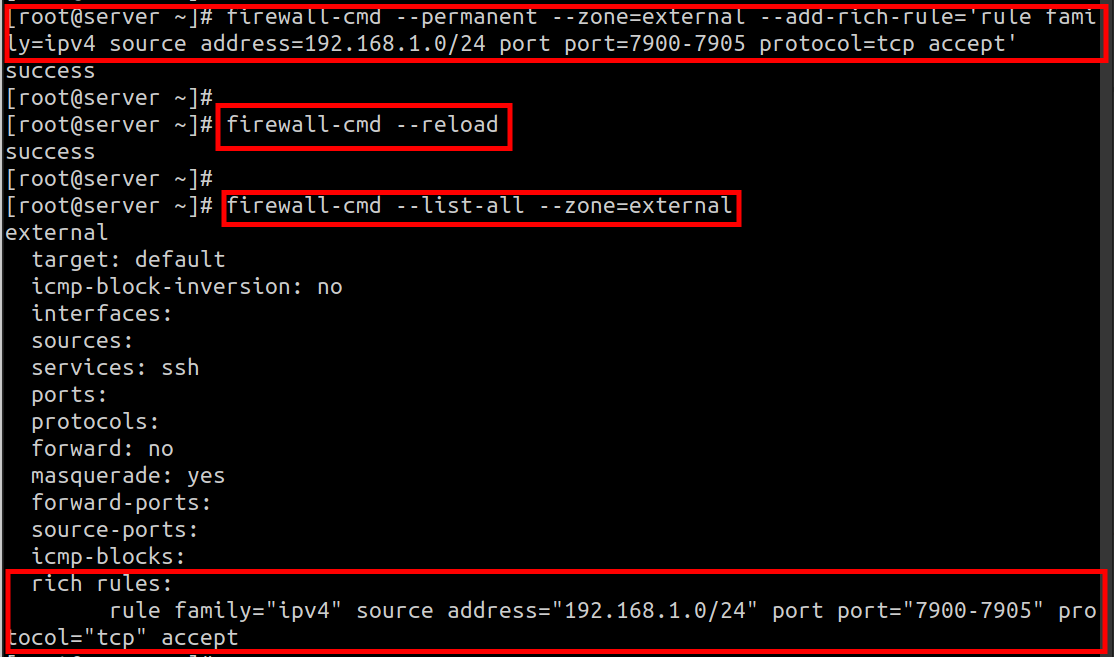
\includegraphics[scale=.3]{content/chapter2/images/zones12.png}
			\caption{Sample output}
			\label{fig:command_prompt10}
		\end{figure}
		
	\end{enumerate}

	\end{itemize}
	
\end{flushleft}

\newpage


\subsection{Port forwarding}

\begin{flushleft}

\begin{itemize}
	\item Port forwarding is a form of \textbf{NAT} (Network Address Translation). 
	\item With port forwarding, traffic of a server is forwarded to a different port on the same machine, or to a port on a different machine. 
	\item This is used \textbf{“hide”} a server behind another machine, or to provide access to a service on an alternate port.
	\item Eg: 
	\begin{itemize}
		\item Ssh server with IP address "192.168.0.108" can configure rich rule such that traffic coming from client address "192.168.0.106" at port 2020 is forwarded to port 22 on ssh server.
	\end{itemize}
	\begin{figure}[h!]
		\centering
		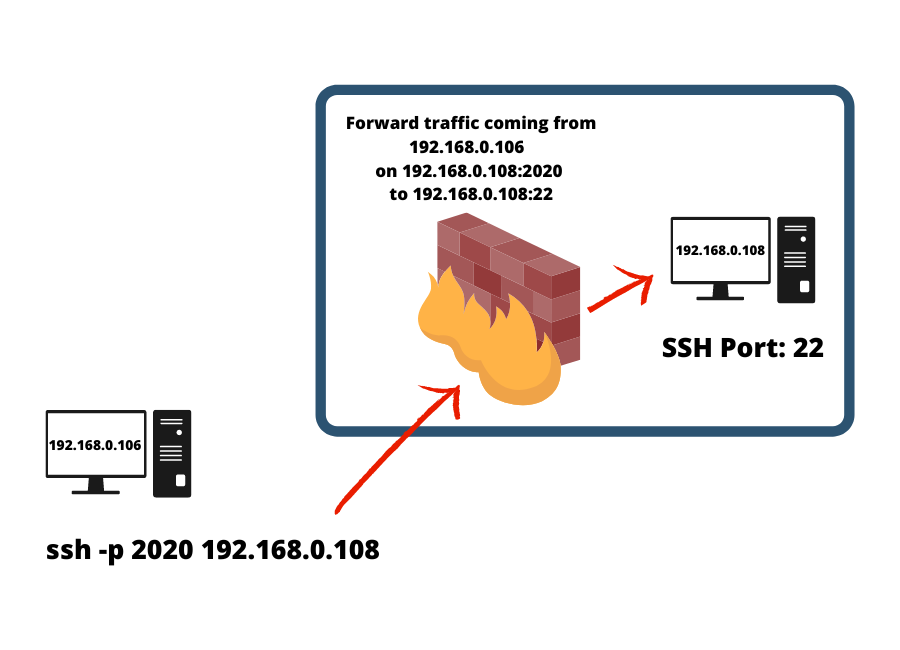
\includegraphics[scale=.52]{content/chapter2/images/port.png}
		\caption{Port forwarding}
		\label{fig:command_prompt12}
	\end{figure}
	
	\begin{tcolorbox}[breakable,notitle,boxrule=-0pt,colback=black,colframe=black]
			\color{green}
			\fontdimen2\font=1em
			\# firewall-cmd --permanent --add-rich-rule 'rule family=ipv4 source address=192.168.0.106/24 forward-port port=2020 protocol=tcp to-port=22'
			\newline
			\newline
			\# firewall-cmd --reload
			\fontdimen2\font=4pt
	\end{tcolorbox}
		
	
\end{itemize}

	
\end{flushleft}

\newpage






\subsection{Practice}
%
\begin{flushleft}

\begin{itemize}
	\item Port forwarding is a form of \textbf{NAT} (Network Address Translation). 
	\item With port forwarding, traffic of a server is forwarded to a different port on the same machine, or to a port on a different machine. 
	\item This is used \textbf{“hide”} a server behind another machine, or to provide access to a service on an alternate port.
	\item Eg: 
	\begin{itemize}
		\item Ssh server with IP address "192.168.0.108" can configure rich rule such that traffic coming from client address "192.168.0.106" at port 2020 is forwarded to port 22 on ssh server.
	\end{itemize}
	\begin{figure}[h!]
		\centering
		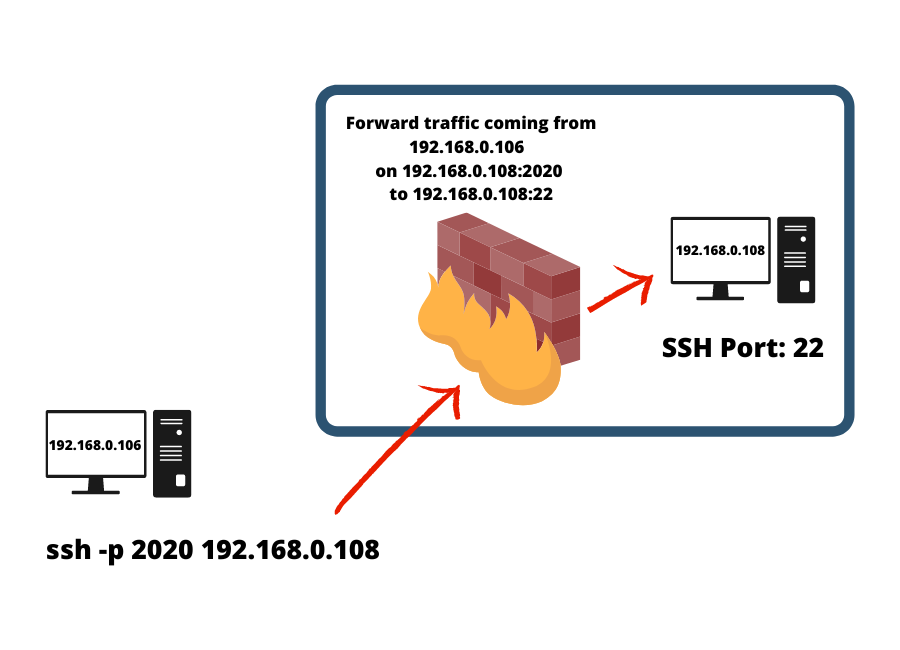
\includegraphics[scale=.52]{content/chapter2/images/port.png}
		\caption{Port forwarding}
		\label{fig:command_prompt12}
	\end{figure}
	
	\begin{tcolorbox}[breakable,notitle,boxrule=-0pt,colback=black,colframe=black]
			\color{green}
			\fontdimen2\font=1em
			\# firewall-cmd --permanent --add-rich-rule 'rule family=ipv4 source address=192.168.0.106/24 forward-port port=2020 protocol=tcp to-port=22'
			\newline
			\newline
			\# firewall-cmd --reload
			\fontdimen2\font=4pt
	\end{tcolorbox}
		
	
\end{itemize}

	
\end{flushleft}

\newpage






%-----------------------

%----------------------------------------------------------------------------------------
%	CHAPTER 3
%----------------------------------------------------------------------------------------
\chapterimage{index4.png} % Table of contents heading image
\chapter{Domain Name Server}
%-----------------------
\section{Introduction to DNS}
\setlength{\columnsep}{3pt}
\begin{flushleft}
	\bigskip
	\bigskip
	\begin{tcolorbox}[breakable,notitle,boxrule=1pt,colback=black,colframe=black]
		\color{white}
		\bigskip
		In this section, you are going to learn:
		\begin{enumerate}
			\item \textbf{What is vi/vim editor?}
			\item \textbf{Using vim editor:}
			\begin{itemize}
				\item \textbf{How to move around in the file?}
				\item \textbf{How to searching for text in the file?}
				\item \textbf{How to save or not save the file?}
				\item \textbf{Other related function related to file editing}
			\end{itemize}

		\end{enumerate}	
		\bigskip
		Finally, there will be a \textbf{small excerise} on these topics to check your knowledge.
		\bigskip
	\end{tcolorbox}
	
	
	\bigskip
	\bigskip
	
	\begin{multicols}{2}
		\vspace*{\fill}
		\vspace*{\fill}
		\vspace*{\fill}
		\vspace*{\fill}
		\vspace*{\fill}
		\vspace*{\fill}
		\vspace*{\fill}
		\vspace*{\fill}
		\vspace*{\fill}
		
		\vfill \null
		\columnbreak
		So let's get started....
		
\includegraphics[scale=0.08]{content/linux_section.png}
	\end{multicols}	
	
\end{flushleft}

\newpage


\subsection{What is /etc/hosts file?}
\setlength{\columnsep}{3pt}
\begin{flushleft}
	\bigskip
	\begin{itemize}
		\item Every machine on internet is identified by a numerical address.
		\item It will be very difficult to memorize the numerical address of all the machines in the network. 
		\item To solve the problem, historically, every machine in the network used \textbf{/etc/hosts} file where the name to address mapping was done.
		\item Structure of \textbf{/etc/hosts} file:
		\begin{tcolorbox}[breakable,notitle,boxrule=1pt,colback=pink,colframe=pink]
			\color{black}
			\fontdimen2\font=1em
			\newline
			\fontdimen2\font=4em
			IP-address      FQDN
			\fontdimen2\font=4pt
		\end{tcolorbox}	
	
		Eg:
		
		\begin{tcolorbox}[breakable,notitle,boxrule=-0pt,colback=black,colframe=black]
			\color{green}
			\fontdimen2\font=1em
			\# cat /etc/hosts
			\newline
			\color{white}
			192.168.2.4   server.example.com.
			\newline
			192.168.2.6	  client.example.com.
			\fontdimen2\font=4pt
		\end{tcolorbox}
		
	\end{itemize}
\end{flushleft}

\newpage






\subsection{Problem with /etc/hosts}
\setlength{\columnsep}{3pt}
\begin{flushleft}
	\bigskip
	\begin{itemize}
		\item Every machine on internet needed to be update with newly added server entries in \textbf{/etc/hosts} file.
		\bigskip
		\item There was no kind of notification available for clients to know a new entry has been added.
		\bigskip		
		\item A single \textbf{/etc/hosts} file became large and very large, making it difficult to handle.
	\end{itemize}

	\paragraph{Solution: DNS server or nameservers}
	\begin{itemize}
		\item During the mid 1970's, \textbf{nameservers} came into place. 
		\bigskip
		\item Idea behind \textbf{nameservers} was to solve the problem of resolving hostname to numbers.
		\bigskip
		\item Nameserver, are also known as a \textbf{DNS server}.
		\bigskip
		\item DNS servers are mentioned in \textbf{/etc/resolv.conf} file.		
	\end{itemize}


	\newpage
	\paragraph{/etc/resolv.conf file}
	\begin{itemize}
		\item Lists nameservers that are used for DNS resolution. 
		\item This file contains a lines specifying the \textbf{"search domains"} and up to \textbf{three IP addresses of DNS server}. 
		\item Eg: Below resolv.conf have two \textbf{search domains} and \textbf{three DNS servers}:
		\begin{tcolorbox}[breakable,notitle,boxrule=-0pt,colback=black,colframe=black]
			\color{green}
			\fontdimen2\font=1em
			\# cat /etc/resolv.conf
			\newline
			\color{white}
			search us.mydomain.com mydomain.com
			\newline
			nameserver 192.168.154.3
			\newline
			nameserver 192.168.154.4
			\newline
			nameserver 10.216.106.3
			\fontdimen2\font=4pt
		\end{tcolorbox}
		\item If you are using DHCP, this file is automatically populated with DNS record issued by DHCP server.
		
	\end{itemize}

	\newpage
	\paragraph{/etc/nsswitch.conf file}
	\begin{itemize}
		\item This file defines, "Who should be consulted first for resolution of domain name, a DNS server or a /etc/hosts file?" 
		\bigskip
		\item Eg: Configuration setting \textbf{"hosts: files dns"} in this file means:
		\begin{itemize}
			\item \textbf{/etc/hosts} file will be checked first for resolution.
			\item If domain is still un-resolvable, DNS will then be consulted.
		\end{itemize}
		\begin{figure}[h!]
			\centering
			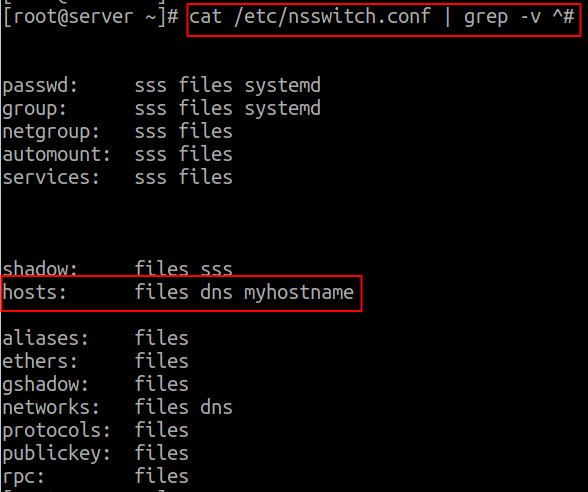
\includegraphics[scale=.45]{content/chapter3/images/ns.png}
			\caption{nsswitch file with hosts entry}
			\label{fig:ns}
		\end{figure}
		\item Note that DNS servers are mentioned in \textbf{/etc/resolv.conf}.
	\end{itemize}
	
	
	\newpage
	\bigskip
	\bigskip
	
	\begin{figure}[h!]
		\centering
		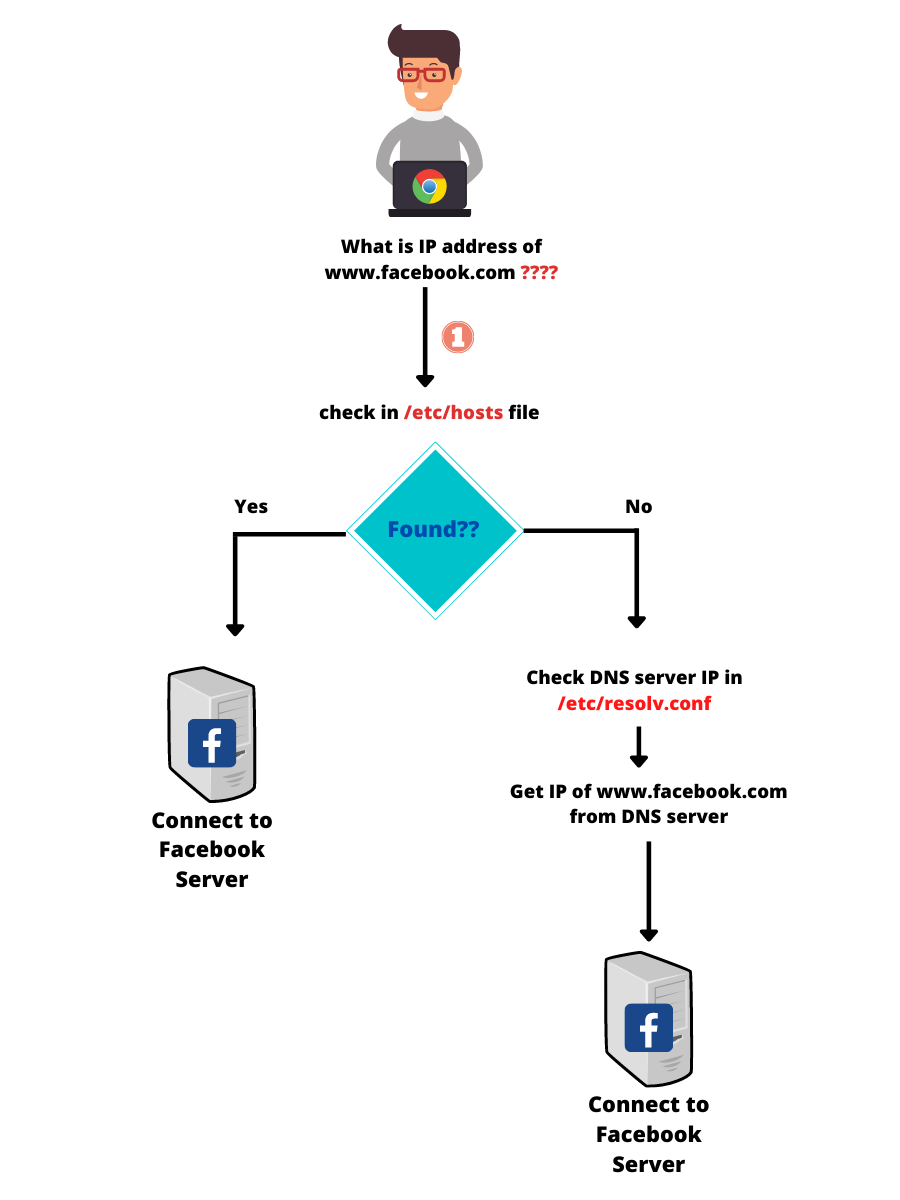
\includegraphics[scale=.6]{content/chapter3/images/hosts.png}
		\caption{Working of /etc/nsswitch.conf}
		\label{fig:dns_s}
	\end{figure}
	


\end{flushleft}

\newpage






\subsection{What is DNS?}
\setlength{\columnsep}{3pt}
\begin{flushleft}
	\bigskip
	\begin{itemize}
		
		\item A DNS server, is also known as a \textbf{nameserver}.
		\item DNS stands for \textbf{D}omain \textbf{N}ame \textbf{S}ystem.
		\item It resolve (translate) \textbf{hostnames to IP addresses} and vice versa. 


		\begin{figure}[h!]
			\centering
			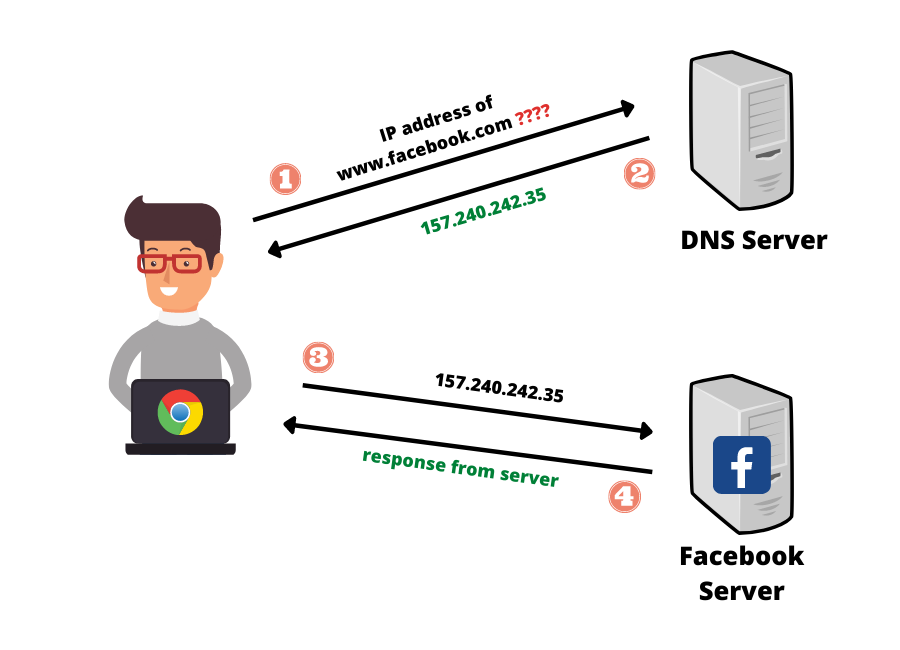
\includegraphics[scale=.6]{content/chapter3/images/dns2.png}
			\caption{DNS server}
			\label{fig:dns_server}
		\end{figure}
	
	\end{itemize}
\end{flushleft}

\newpage






\subsection{The DNS hierarchy}

\begin{flushleft}
	\bigskip
	\begin{figure}[h!]
		\centering
		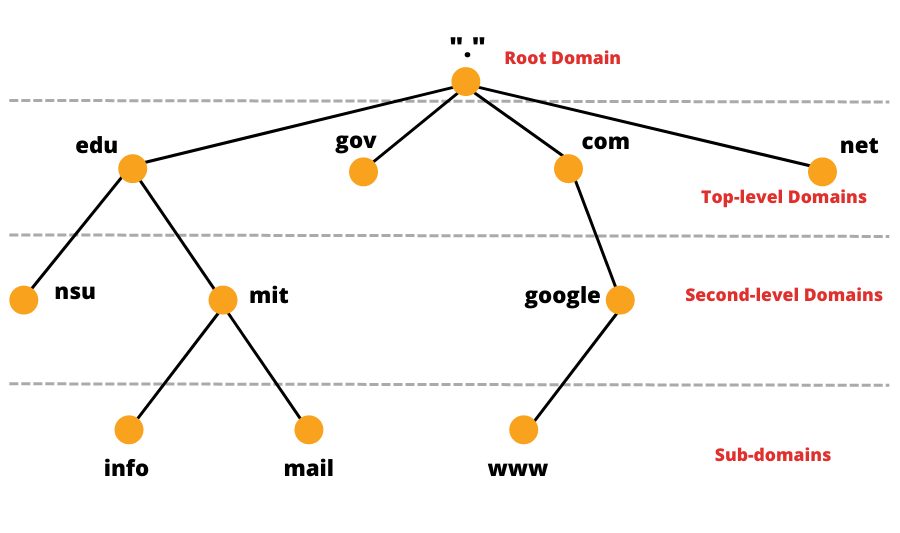
\includegraphics[scale=.6]{content/chapter3/images/dns.png}
		\caption{DNS Hierarchy}
		\label{fig:dns_heir}
	\end{figure}
	\begin{itemize}
		\item \textbf{What is domain?}
		\begin{itemize}
			\item A domain name is an easy-to-remember address used to access websites. 
		\end{itemize}
		\item A domain consist of:
		\begin{itemize}
			\item The \textbf{root-level domain} at the top
			\item The \textbf{top-level domains}(TLD) underneath it
			\item Followed by \textbf{second-level domains}
			\item Finally \textbf{sub-domains}.
		\end{itemize}
		Let's see each of these in detail

		\newpage
		
		
		\item \textbf{What is root-level domain?}
		\bigskip
		\begin{itemize}
			\item Root domain is the highest hierarchical level of the Internet.
			\bigskip
			\item When any DNS server is asked for an information which it does not have, the first thing that DNS server does is asking one of the (.)root name server.
			\begin{figure}[h!]
				\centering
				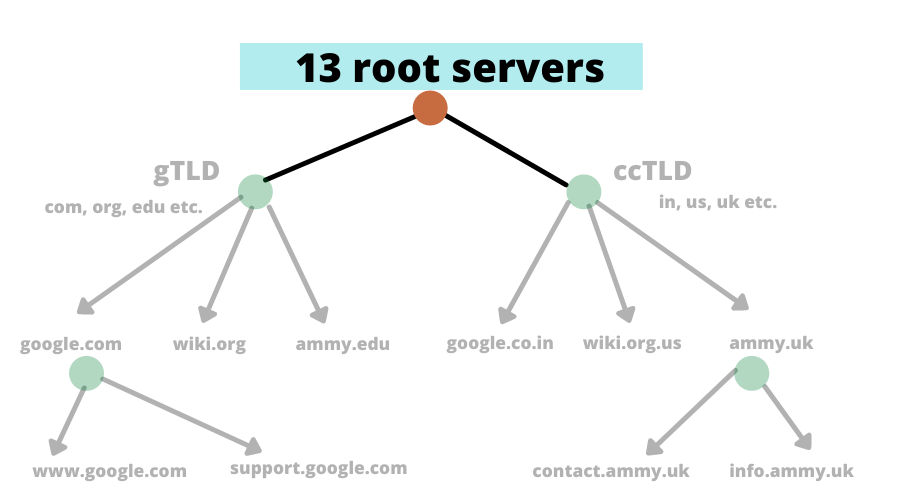
\includegraphics[scale=.5]{content/chapter3/images/page1.png}
				\caption{13 root servers}
				\label{fig:root_servers}
			\end{figure}		
			\item There are 13 root name servers as follows:
			\begin{itemize}
				\item a.root-servers.net.
				\item b.root-servers.net.
				\item c.root-servers.net.
				\item d.root-servers.net.
				\item e.root-servers.net.
				\item f.root-servers.net.
				\item g.root-servers.net.
				\item h.root-servers.net.
				\item i.root-servers.net.
				\item j.root-servers.net.
				\item k.root-servers.net.
				\item l.root-servers.net.
				\item m.root-servers.net.
			\end{itemize}
		\end{itemize}
		\newpage
		
			
		
		\newpage
		\item \textbf{What is TLD?}
		\bigskip
		\begin{itemize}
			\item TLDs tell users the general purpose of the service behind the domain name. 
			\bigskip
			\item Types of TLD:
			\begin{itemize}
				\item Generic TLDs (gTLDs) like \textbf{.com}, \textbf{.edu}, \textbf{.net}, etc.
				\item Country code TLDs (ccTLDs) like \textbf{.us}, \textbf{.uk}, \textbf{.ru}, \textbf{.in}, etc. 
			\end{itemize}  
		
			\begin{figure}[h!]
				\centering
				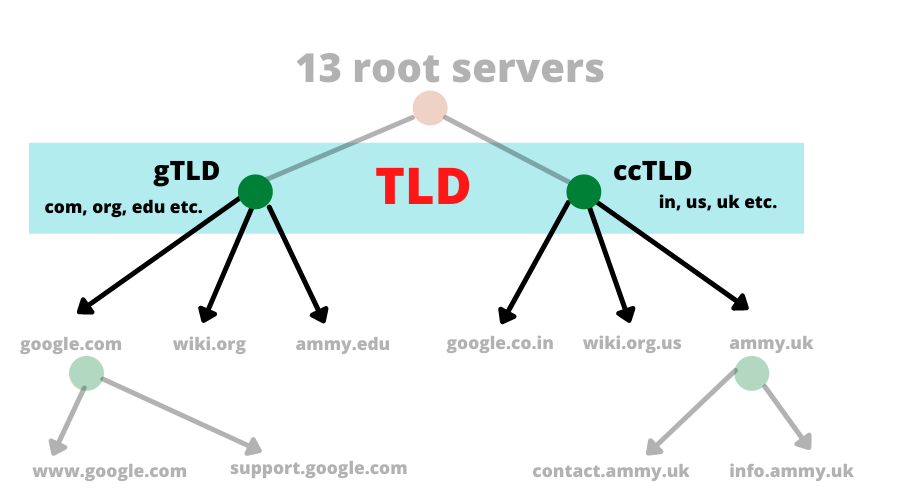
\includegraphics[scale=.5]{content/chapter3/images/page2.png}
				\caption{TLD types}
				\label{fig:tld}
			\end{figure}		
			\bigskip
			\item List of TLDs: https://data.iana.org/TLD/tlds-alpha-by-domain.txt
		\end{itemize}

		\newpage
		\item \textbf{What is second level domain?}
		\bigskip
		
		\begin{itemize}
			\item This is where domain holders put the brand name, project name, organization name or other familiar identifier for users.
			
			\begin{figure}[h!]
				\centering
				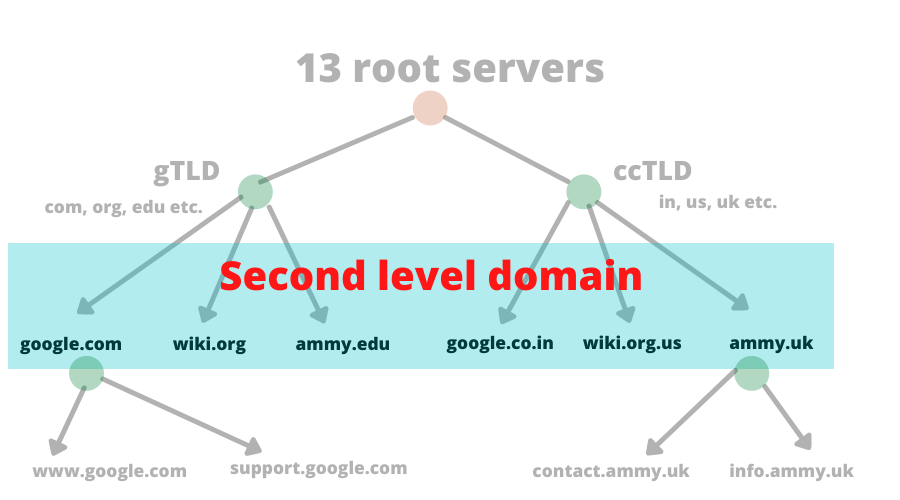
\includegraphics[scale=.5]{content/chapter3/images/page3.png}
				\caption{Second level domain}
				\label{fig:sec_domain}
			\end{figure}		
			
			\item Eg: For amazon.com, \textbf{amazon} is second level domain.
		\end{itemize}
	
		\newpage		
		\item \textbf{What is subdomain?}
		\bigskip
		\begin{itemize}
			\item It is additional information added to the front of website's domain name. 
			\bigskip
			\item It organizes the content for website.
			
			\begin{figure}[h!]
				\centering
				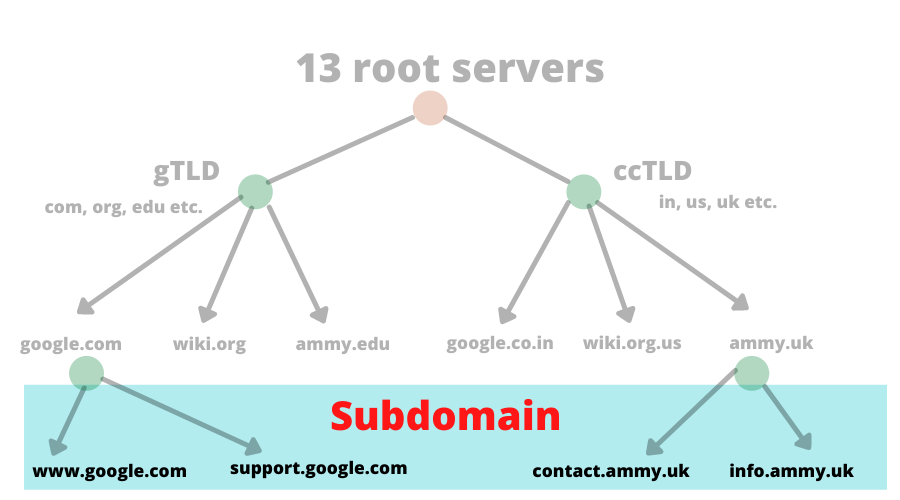
\includegraphics[scale=.5]{content/chapter3/images/page4.png}
				\caption{Subdomain}
				\label{fig:subdomain}
			\end{figure}		
							
		\end{itemize}
	
		\newpage
		
		\paragraph{Command examining the DNS query structure}
		\bigskip
		\item \textbf{dig +trace domainname}: Understand the entire flow of the query.
		\bigskip
		\begin{tcolorbox}[breakable,notitle,boxrule=-0pt,colback=black,colframe=black]
			\color{green}
			\fontdimen2\font=1em
			\# dig +trace google.com
			\fontdimen2\font=4pt
		\end{tcolorbox}
		Eg:
		\begin{figure}[h!]
			\centering
			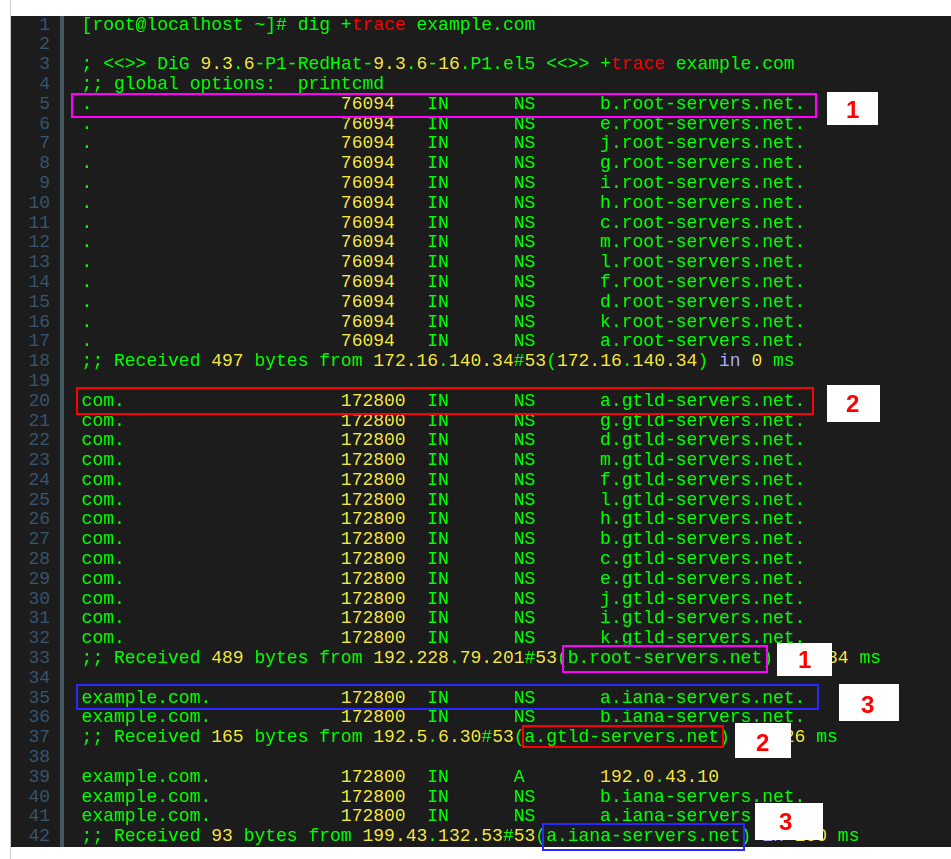
\includegraphics[scale=.35]{content/chapter3/images/dig.png}
			\caption{dig command output}
			\label{fig:dig}
		\end{figure}
		
		Understanding dig command output:
		\begin{itemize}
			\item \textbf{/etc/resolv.conf}: Your local dns server (in \textbf{/etc/resolv.conf}), provides with address of the \textbf{13 dns root servers}. 
			\item \textbf{Box 1}: Dig command selects one root server from the 13, to fetch the address of the \textbf{.com TLD servers}. 
			\item \textbf{Box 2}: The root server selected will reply with the \textbf{.com TLD server} addresses.
			\item \textbf{Box 3}: The \textbf{COM GTLD server} replied with IP address of "example.com" which is \textbf{192.0.43.10}.
			
			
		\end{itemize}
		
		
		

	\end{itemize}	
	
\end{flushleft}

\newpage

\subsection{How domain names are assigned?}

\begin{flushleft}

	\begin{itemize}
		\item The \textbf{I}nternet \textbf{C}orporation for \textbf{A}ssigned \textbf{N}ames and \textbf{N}umbers (ICANN) is the ultimate authority for domain-name assignments. 
		\bigskip
		\bigskip
		\item \textbf{Buying a domain name}
		\begin{itemize}
			\item First check if domain you want is available here or not: https://lookup.icann.org/en
			\item If it is available, you cannot "buy a domain name".
			\item You pay for the right to use a domain name for one or more years.
			\item You can renew your right after it's duration is expired.
			\item In simple words, you rent a second-level domain name.
		\end{itemize}
		\bigskip
		\bigskip
		 \item \textbf{How many subdomains are possible for domain name?}
		 \begin{itemize}
		 	\item Owner of domain can create unlimited number of subdomains.
		 	 \item Eg: utexas.edu can have second-level domain like:
		 	\begin{itemize}
		 		\item gslis.utexas.edu
		 		\item computerstore.utexas.edu
		 	\end{itemize}
		 \end{itemize}
		\bigskip
		\bigskip
		 \item \textbf{How big can be a domain name?}
		 \begin{itemize}
		 	\item Each subdomain can have its own subdomains. 
		 	\item Eg: example.subdomains.in.the.domain.utexas.edu.
			\item There can be \textbf{maximum 127 subdomains} in a single domain name. 
			\item Maximum size of each subdomain is \textbf{63} characters.
		 \end{itemize}  
		
		

		
	\end{itemize}








\end{flushleft}
\newpage
\subsection{Practice}
%
\begin{flushleft}

\begin{itemize}
	\item Port forwarding is a form of \textbf{NAT} (Network Address Translation). 
	\item With port forwarding, traffic of a server is forwarded to a different port on the same machine, or to a port on a different machine. 
	\item This is used \textbf{“hide”} a server behind another machine, or to provide access to a service on an alternate port.
	\item Eg: 
	\begin{itemize}
		\item Ssh server with IP address "192.168.0.108" can configure rich rule such that traffic coming from client address "192.168.0.106" at port 2020 is forwarded to port 22 on ssh server.
	\end{itemize}
	\begin{figure}[h!]
		\centering
		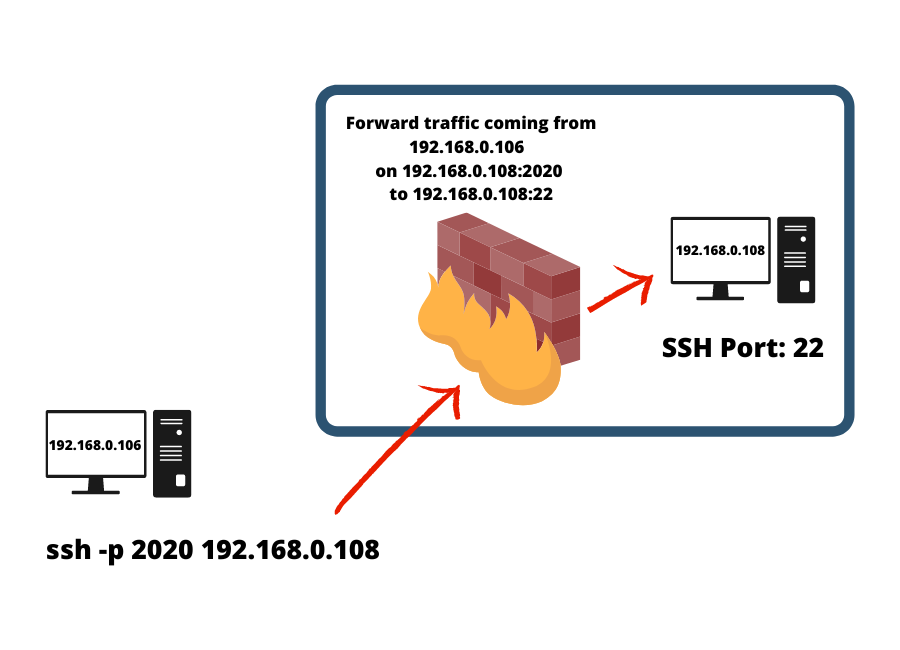
\includegraphics[scale=.52]{content/chapter2/images/port.png}
		\caption{Port forwarding}
		\label{fig:command_prompt12}
	\end{figure}
	
	\begin{tcolorbox}[breakable,notitle,boxrule=-0pt,colback=black,colframe=black]
			\color{green}
			\fontdimen2\font=1em
			\# firewall-cmd --permanent --add-rich-rule 'rule family=ipv4 source address=192.168.0.106/24 forward-port port=2020 protocol=tcp to-port=22'
			\newline
			\newline
			\# firewall-cmd --reload
			\fontdimen2\font=4pt
	\end{tcolorbox}
		
	
\end{itemize}

	
\end{flushleft}

\newpage






\section{DNS concepts}

\paragraph{Welcome}
Welcome guys! We are glad to have you here.

\newpage
\subsection{Types of DNS server}

\setlength{\columnsep}{3pt}
\begin{flushleft}
	\bigskip
	\begin{itemize}
		\item \textbf{Authoritative nameserver}:
		\begin{itemize}
			\item An authoritative nameserver has the original settings for domain name.
			\item This is where the domain administrator has configured the DNS records for a domain. 
			
			\begin{figure}[h!]
				\centering
				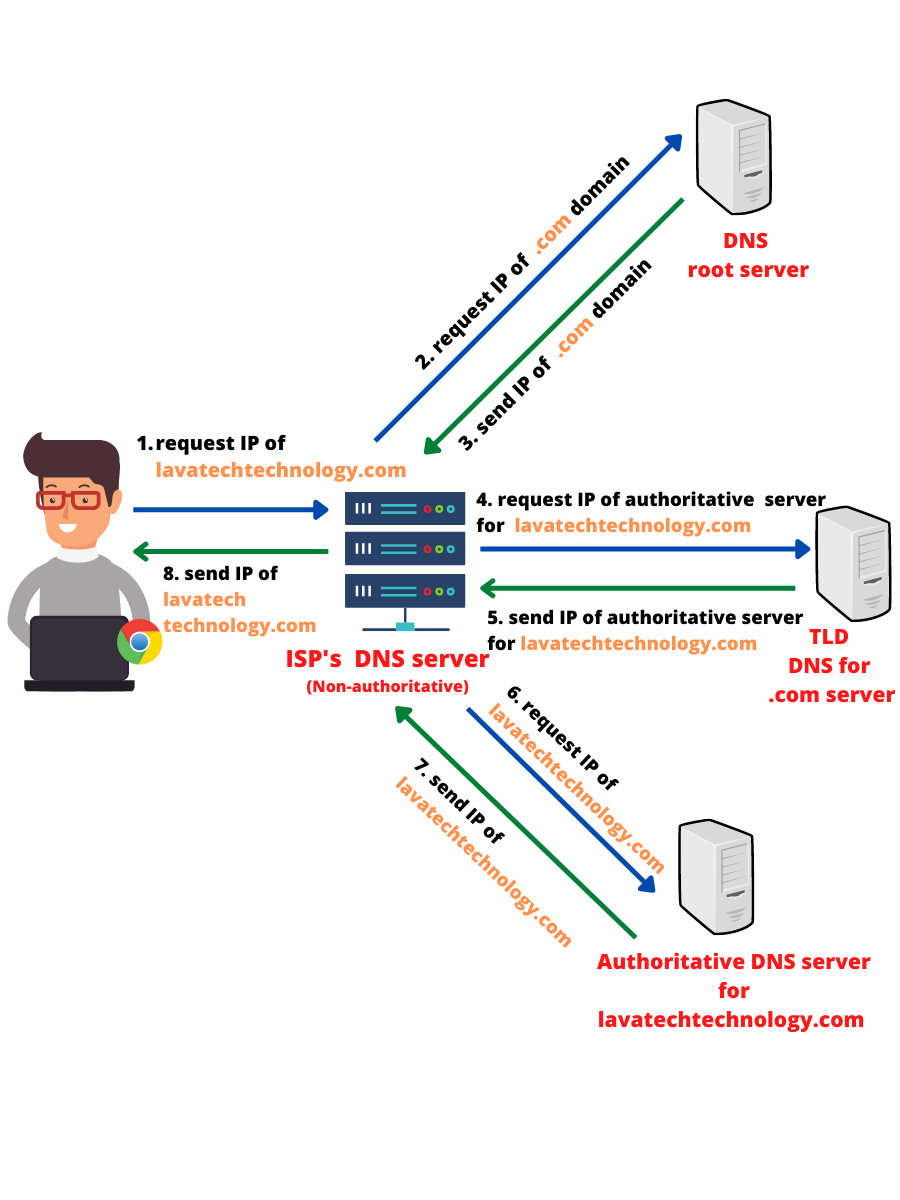
\includegraphics[scale=.48]{content/chapter3/images/auth.png}
				\caption{DNS Hierarchy}
				\label{fig:dns_heir}
			\end{figure}
			\newpage
			\item Find authoritative DNS server for any domain:
			\begin{tcolorbox}[breakable,notitle,boxrule=0pt,colback=pink,colframe=pink]
				\color{black}
				\fontdimen2\font=1em
				Syntax: dig +short NS <domain name>
				\fontdimen2\font=4pt
			\end{tcolorbox}
			Eg:
			\begin{tcolorbox}[breakable,notitle,boxrule=-0pt,colback=black,colframe=black]
				\color{green}
				\fontdimen2\font=1em
				\# dig +short NS lavatechtechnology.com
				\newline
				\color{white}
				ns06.domaincontrol.com.
				\newline
				ns05.domaincontrol.com.
				\fontdimen2\font=4pt
			\end{tcolorbox}
			
			or 
			\begin{tcolorbox}[breakable,notitle,boxrule=0pt,colback=pink,colframe=pink]
				\color{black}
				\fontdimen2\font=1em
				Syntax: host -t ns <domain name>
				\fontdimen2\font=4pt
			\end{tcolorbox}
			Eg:
			\begin{tcolorbox}[breakable,notitle,boxrule=-0pt,colback=black,colframe=black]
				\color{green}
				\fontdimen2\font=1em
				\# host -t ns lavatechtechnology.com
				\newline
				\color{white}
				lavatechtechnology.com name server ns06.domaincontrol.com.
				\newline
				lavatechtechnology.com name server ns05.domaincontrol.com.
				\fontdimen2\font=4pt
			\end{tcolorbox}
			
			\bigskip
			\item Using \textbf{nslookup} (\textbf{N}ame \textbf{S}erver lookup) command, confirm if the domain name is resolved using the authoritative nameserver.
			\begin{tcolorbox}[breakable,notitle,boxrule=0pt,colback=pink,colframe=pink]
				\color{black}
				\fontdimen2\font=1em
				Syntax: nslookup <domain-name> <nameserver>
				\fontdimen2\font=4pt
			\end{tcolorbox}
			
			\begin{figure}[h!]
				\centering
				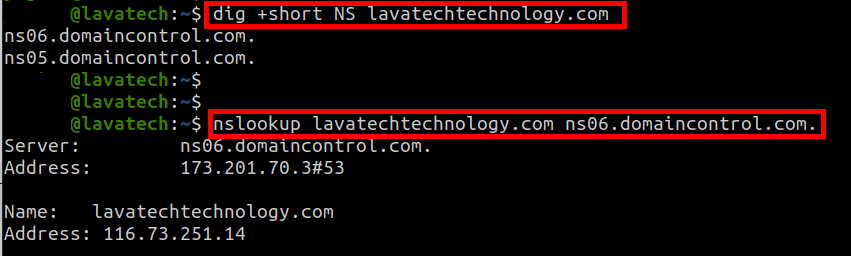
\includegraphics[scale=.35]{content/chapter3/images/ans.png}
				\caption{Sample output}
				\label{fig:dns_heir3}
			\end{figure}			
		
		\end{itemize}
		
		\newpage
		\item \textbf{Non-authoritative nameserver}:
		\begin{itemize}
			\item Non-authoritative name servers do not contain original source files of domain’s zone. 
			\item They have a \textbf{cache file} for the domains that is constructed from all the DNS lookups done previously. 
			\item If a DNS server responded for a DNS query which doesn’t have original file is known as a Non-authoritative answer.
			\item Find non-authoritative DNS server for any domain:
			\begin{tcolorbox}[breakable,notitle,boxrule=0pt,colback=pink,colframe=pink]
				\color{black}
				\fontdimen2\font=1em
				Syntax: nslookup <domain-name>
				\fontdimen2\font=4pt
			\end{tcolorbox}
			Eg:
			\begin{tcolorbox}[breakable,notitle,boxrule=-0pt,colback=black,colframe=black]
				\color{green}
				\fontdimen2\font=1em
				\# nslookup lavatechtechnology.com
				\fontdimen2\font=4pt
			\end{tcolorbox}
			
			\begin{figure}[h!]
				\centering
				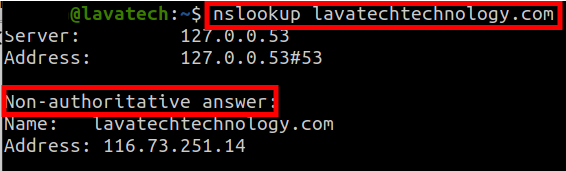
\includegraphics[scale=.5]{content/chapter3/images/ns1.png}
				\caption{Sample output}
				\label{fig:dns_heir4}
			\end{figure}			

			\begin{figure}[h!]
				\centering
				\includegraphics[scale=.6]{content/chapter3/images/ns2.png}
				\caption{Sample output}
				\label{fig:dns_heir5}
			\end{figure}			
			
		\end{itemize}
		
		
		
		\item \textbf{}:
	
	\end{itemize}
\end{flushleft}

\newpage






\subsection{8.8.8.8 DNS server}
\setlength{\columnsep}{3pt}
\begin{flushleft}
	\bigskip
	\begin{itemize}
		\item Can I use an 8.8 8.8 DNS?
		\item This is the public DNS server of Google and basically means that Google is the provider of the DNS and is responsible for the maintenance of the service. This DNS can be used by anyone on the internet.
	
	\end{itemize}
\end{flushleft}

\newpage






\subsection{Zones in DNS}
\setlength{\columnsep}{3pt}
\begin{flushleft}

	\paragraph{What is DNS zone?}

	\begin{itemize}
		\item The DNS is broken up into many different zones. 
		\item \textbf{DNS zones encompass all records for a domain. }
		\item Eg: A zone for xzy.com would contain records such as www.xzy.com, support.xyz.com etc.
			\begin{figure}[h!]
			\centering
			\includegraphics[scale=.55]{content/chapter3/images/zone.png}
			\caption{DNS zone}
			\label{fig:dns_heir32}
		\end{figure}
	\end{itemize}

	\paragraph{What is zone file?}
	\begin{itemize}
		\item A DNS zone file is a text file that maps domain names and IP addresses.
		\item They are human-readable and editable. 
		
	\end{itemize}
\end{flushleft}

\newpage






\subsection{Forward \& Reverse zone}
\setlength{\columnsep}{3pt}
\begin{flushleft}
	\bigskip
	\paragraph{Forward Lookup zone}
	\begin{itemize}
		\item Converts a \textbf{domain name to an IP address} or another name. 
		\item This zone contains all the records of domain names to their IP addresses.
	\end{itemize}

	\paragraph{Reverse Lookup zone}
	
	\begin{itemize}
		\item Converts a \textbf{an IP address to domain name}.
		\item This zone contains all the records of IP addresses to their domain names.
	\end{itemize}

	\begin{figure}[h!]
		\centering
		\includegraphics[scale=.6]{content/chapter3/images/reverse.png}
		\caption{Forward \& Reverse DNS Lookup}
		\label{fig:dns_heir76}
	\end{figure}

\end{flushleft}

\newpage






\subsection{Forward zone file}
\setlength{\columnsep}{3pt}
\begin{flushleft}
	\bigskip
	\begin{itemize}

		\begin{figure}[h!]
			\centering
			\includegraphics[scale=.4]{content/chapter3/images/zone1.png}
		\end{figure}
		\item \$TTL – DNS TTL (time to live) is a setting that tells the DNS resolver how long to cache a query before requesting a new one.

		\newpage
		\begin{figure}[h!]
			\centering
			\includegraphics[scale=.4]{content/chapter3/images/zone2.png}
		\end{figure}
		\begin{tcolorbox}[breakable,notitle,boxrule=1pt,colback=pink,colframe=pink]
			\color{black}
			\fontdimen2\font=2em
			Syntax: 

			\newline
			@   IN  SOA  @  hostmaster-email (
			\newline
			serial-number
			\newline
			time-to-refresh
			\newline
			time-to-retry
			\newline
			time-to-expire
			\newline
			minimum-TTL)
			\fontdimen2\font=4pt
		\end{tcolorbox}	
		
		\begin{itemize}
			\item @ means domain-name
			\item IN: Stands for Internet
			\item SOA: The DNS ‘start of authority’ (SOA) record stores important information about a domain or zone such as the email address of the administrator, when the domain was last updated, and how long the server should wait between refreshes.
			\item 
			
		\end{itemize}
		
		\newpage
		\begin{figure}[h!]
			\centering
			\includegraphics[scale=.4]{content/chapter3/images/zone3.png}
		\end{figure}
		\begin{tcolorbox}[breakable,notitle,boxrule=1pt,colback=pink,colframe=pink]
			\color{black}
			\fontdimen2\font=2em
			Syntax: 
			\newline
			\color{blue}
			@   IN  SOA  @  hostmaster-email (
			\newline
			serial-number
			\newline
			time-to-refresh
			\newline
			time-to-retry
			\newline
			time-to-expire
			\newline
			minimum-TTL)
			\fontdimen2\font=4pt
		\end{tcolorbox}	
		\begin{itemize}
			\item The DNS ‘start of authority’ (SOA) record stores important information about a domain or zone such as the email address of the administrator, when the domain was last updated, and how long the server should wait between refreshes.
		\end{itemize}			
		
	\end{itemize}
\end{flushleft}

\newpage







\subsection{DNS RESOURCE RECORDS}
\setlength{\columnsep}{3pt}
\begin{flushleft}

	\paragraph{What is DNS zone?}

	\begin{itemize}
		\item The DNS is broken up into many different zones. 
		\item \textbf{DNS zones encompass all records for a domain. }
		\item Eg: A zone for xzy.com would contain records such as www.xzy.com, support.xyz.com etc.
			\begin{figure}[h!]
			\centering
			\includegraphics[scale=.55]{content/chapter3/images/zone.png}
			\caption{DNS zone}
			\label{fig:dns_heir32}
		\end{figure}
	\end{itemize}

	\paragraph{What is zone file?}
	\begin{itemize}
		\item A DNS zone file is a text file that maps domain names and IP addresses.
		\item They are human-readable and editable. 
		
	\end{itemize}
\end{flushleft}

\newpage







%-----------------------

%----------------------------------------------------------------------------------------
%	CHAPTER 4
%----------------------------------------------------------------------------------------
\chapterimage{index5.png} % Table of contents heading image
\chapter{Samba Server}
%-----------------------
%-----------------------

%----------------------------------------------------------------------------------------
%	CHAPTER 5
%----------------------------------------------------------------------------------------
\chapterimage{index6.png} % Table of contents heading image
\chapter{NFS Server}
%-----------------------

%-----------------------

%----------------------------------------------------------------------------------------
%	CHAPTER 6
%----------------------------------------------------------------------------------------
\chapterimage{index7.png} % Table of contents heading image
\chapter{Teaming and Bridging}
%-----------------------

%-----------------------

%----------------------------------------------------------------------------------------
%	CHAPTER 7
%----------------------------------------------------------------------------------------
\chapterimage{index8.png} % Table of contents heading image
\chapter{ISCSI Server}
%%%%%-----------------------


%%%%
%%%%%-----------------------
%%%%
%%%%
%%%%%----------------------------------------------------------------------------------------
%%%%%	CHAPTER 8
%%%%%----------------------------------------------------------------------------------------
\chapterimage{index9.png} % Table of contents heading image
\chapter{Apache Server}
%%%%%-----------------------


%----------------------------------------------------------------------------------------
%	BIBLIOGRAPHY
%----------------------------------------------------------------------------------------

%\chapter*{Bibliography}
%\addcontentsline{toc}{chapter}{\textcolor{ocre}{Bibliography}} % Add a Bibliography heading to the table of contents
%
%%------------------------------------------------
%
%\section*{Articles}
%\addcontentsline{toc}{section}{Articles}
%\printbibliography[heading=bibempty,type=article]
%
%%------------------------------------------------
%
%\section*{Books}
%\addcontentsline{toc}{section}{Books}
%\printbibliography[heading=bibempty,type=book]
%
%%----------------------------------------------------------------------------------------
%%	INDEX
%%----------------------------------------------------------------------------------------
%
%\cleardoublepage % Make sure the index starts on an odd (right side) page
%\phantomsection
%\setlength{\columnsep}{0.75cm} % Space between the 2 columns of the index
%\addcontentsline{toc}{chapter}{\textcolor{ocre}{Index}} % Add an Index heading to the table of contents
%\printindex % Output the index

%----------------------------------------------------------------------------------------


\end{document}


